\documentclass[oneside]{mgr}

\usepackage[utf8]{inputenc}
\usepackage[T1]{fontenc}

\usepackage{graphicx}
%\usepackage{subfigure}
\usepackage{caption}
\usepackage{subcaption}
\usepackage{psfrag}
\usepackage{rotating}


\usepackage{amsmath}
\usepackage{amsfonts}
\usepackage{amsthm}
\usepackage{breqn}

\usepackage{supertabular}
\usepackage{array}
\usepackage{tabularx}
\usepackage{hhline}

\usepackage{multicol}
\usepackage{multirow}
\usepackage{hyperref}

%\usepackage{showlabels} %dodaje z~boku etykiety

\newtheorem{theorem}{Twierdzenie}[section]
\theoremstyle{definition}
\newtheorem{definition}{Definicja}[section]

\newcommand{\ud}{\mathrm{d}}
\newcommand{\rot}{\mathrm{Rot}}
\newcommand{\tr}{\mathrm{Trans}}

\title{Control algorithms of a skid-steering mobile robot}
\engtitle{Algorytmy sterowania robota mobilnego poruszającego się z poślizgami}
\author{Paweł Bogner}
\supervisor{prof. dr hab. inż. Krzysztof Tchoń, K-7}

\field{Automatyka~i~Robotyka~(AIR)}
\specialisation{Robotyka~(ARR)}

\begin{document}
\maketitle

\tableofcontents

%\newgeometry{top=3cm}
\chapter{Introduction}
%\vspace{-0.7cm}
The problem of control of skid-steering mobile robots is a very complex issue. 
The main difficulty is to create an adequate model the phenomenon of friciton. 
There has been many different attempts to describe it.
For instance, the authors of \cite{caracciolo1999trajectory} use the Coulomb friction model limited to the low velocities.
Apart from that, the longitudinal skid was neglected. The approach presented in this paper is different.
The assumption is that the slips are possible in both directions, lateral and longitudinal.
This is similar to the models used in automotive literature \cite{pacejka2005tyre}.
All slips are allowed, but the impact of them to the model may be suppressed by tuning the
parameters properly. 

When it comes to the friction model idea used in this thesis,
it is based on the velocity of the slip derived
from the Pfaffian matrix. %TODO cite 
Two types of models have been considered here: the linear and the discontinuous model.
The linear friction force model is analogous to the mass on the spring. In that case the friciton
force is proportional to the value of the slip, like the spring reaction force is proportional
to the displacement from the equilibrium position. The second model idea bases on the first one,
but includes a modification in order to reflect the fact of losing the traction. Such a change
consists in switching the friction coefficient dependently on the value of the slip.

Skid-steering systems may be considered on two levels --- kinematic and dynamic.
The kinematic model may be derived basing on the motion constraints in the Pfaffian form, which may lead
to a nonholonomic system. This can be extended to include dynamics, using d'Alembert principle.

Motion planning plays an important part in robot control. This is usually the first step of solving
a certain control problem. It is not enough to use a good control algorithm for path following. The fundamental
issue is determining the path or the trajectory to follow. There are many motion planning methods,
such as steering using sinusoids for chained systems \cite{murray1993nonholonomic} or rapidly-exploring random trees for nonholomic systems
with obstacles on the scene \cite{lavalle2000rapidly}. The planning algorithm presented in this paper,
the endogenous configuration approach, can be applied for mobile manipulators, regarding the
mobile platform on dynamic level and the kinematics of the manipulator arm. It has been extensively
tested using RobRex mobile manipulator as a controlled model using different
friction coefficients configurations.

The thesis of this work is that endogenous configuration approach may be used for
motion planning of skid-steering mobile manipulators, including the dynamics of the platform.

The layout of this thesis is as follows. Chapter \ref{ch:model} presents the models of studied
objects: the unicycle and RobRex mobile manipulator. Chapter \ref{ch:endogen} introduces the endogenous
configuration space approach to motion planning problem. In chapter \ref{ch:simul}, there are collected
the results of the simulations of the objects mentioned above, with application of the motion
planning algorithm. Chapter \ref{ch:concl} summarizes the whole study.
%\restoregeometry

\chapter{Models}
\label{ch:model}
In this thesis two different models will be taken into consideration: the unicycle model with system dynamics and the RobRex mobile manipulator with platform dynamics and arm kinematics.
\section{Unicycle}
This is the model of the simplest robotic system --- a unicycle.
The object is modelled as a solid disc with two control inputs:
linear acceleration and angular acceleration with respect to the vertical axis.
Let $x$ and $y$ denote two position coordinates, $\phi$ --- the orientation
and $\theta$ --- the angle of rotation. 
In order to preserve dimensional consistency define the configuration vector in the following way:
$w = (x, y, \phi R, \theta R)^T$, where $R$ is the radius of the wheel.

The equation of motion can be presented
in the form $Q(w)\ddot w =F(w, \dot w)+Bu$. This can be easily acquired with usage of Euler-Lagrange formalism. The inertia matrix is $Q(w)=\mathrm{diag}\left\{m, m, \frac{I_\phi}{R^2}, \frac{I_\theta}{R^2}\right\}$ and the input matrix is $B=\begin{bmatrix}
0_{2 \times 2} & I_2
\end{bmatrix}^T$, where $m$ is wheel mass and $I_\phi=\frac{1}{4}mR^2$, $I_\theta=\frac{1}{2}mR^2$.

When it comes to slips reaction forces, the Pfaffian matrix needs to be defined sa
\begin{equation}
H(w)=\begin{bmatrix}
-\sin\phi & \cos\phi & 0 & 0\\
\cos\phi & \sin\phi & 0 & -1
\end{bmatrix}=\begin{bmatrix}
H^1(w)\\
H^2(w)
\end{bmatrix}.
\end{equation}
The slips can be calculated as follows: the lateral slip $s_\perp=H^1(w)\dot w$ and the longitudinal slip $s_\parallel=H^2(w)\dot w$. With this quantities, the slip reaction forces may be defined as 
\begin{equation}
F(w, \dot w)=mg\epsilon s_\perp\frac{H^{1T}(w)}{||H^{1T}(w)||} + mg\tau s_\parallel\frac{H^{2T}(w)}{||H^{2T}(w)||},
\end{equation}
where $g$ is gravitational acceleration, $\epsilon$ and $\tau$ are lateral and longitudinal friction coefficients, respectively.

Transforming the system into a standard control form we finally obtain
\begin{equation}
\frac{\ud}{\ud t}\begin{pmatrix}
w \\ \dot w
\end{pmatrix}
 = 
 \begin{bmatrix}
 \dot w \\ Q^{-1}(w)F(w, \dot w)
 \end{bmatrix}+\begin{bmatrix}
 0_{4\times 2} \\ Q^{-1}(w)B
 \end{bmatrix}.
\end{equation}
\section{RobRex mobile manipulator}
The model consists of two parts: a mobile platform and a manipulator. The platform has got four fixed-axis wheels, which are actuated with two motors --- the wheels on both sides are coupled. The schematic structure of the vehicle is shown in figure ... %TODO
The manipulator is mounted on the platform above the centre of the front wheel axis.
\subsection{Mobile platform}
Let $w\in \mathbb{R}^5$ be the configuration of the platform, where
$w=(x, y, a\phi, R\theta_1, R\theta_2)$.  
The dynamics model of the cart is represented in the standard form used in robotics
\begin{equation}
\label{eq:std_mdl}
P(w)\ddot w + D(w, \dot w) = F(w, \dot w) + Bu.
\end{equation}
The elaborate model derivation can be found in \cite{coupled}. 
The elements of \eqref{eq:std_mdl} are equal to
\begin{align}
P(w) &= \begin{bmatrix}
Q_{11} & 0 & \frac{Q_{13}}{a} & 0 & 0\\
0 & Q_{22} & \frac{Q_{23}}{a} & 0 & 0\\
\frac{Q_{13}}{a} & \frac{Q_{23}}{a} & \frac{Q_{33}}{a} & 0 & 0\\
0 & 0 & 0 & \frac{Q_{44}}{R^2} & 0 \\
0 & 0 & 0 & 0 & \frac{Q_{55}}{R^2}
\end{bmatrix}, & 
D(w, \dot w) &= \frac{\dot w_3^2}{a^2}\begin{pmatrix}
-Q_{23} & Q_{13} & 0 & 0 & 0
\end{pmatrix}^T.
\end{align}
The components of the above equations are
\begin{align}
Q_{11} = Q_{22} &= m_p+4m_w,\\
Q_{44} = Q_{55} &= 2I_{w33},\\
Q_{13} &= -m_p(a_{p1}\sin\frac{w_3}{a}+a_{p2}\cos\frac{w_3}{a})- 2m_wa\sin\frac{w_3}{a},\\
Q_{23} &=  m_p(a_{p1}\cos\frac{w_3}{a}-a_{p2}\sin\frac{w_3}{a})+ 2m_wa\cos\frac{w_3}{a},\\
Q_{33} &= I_{p33}+m_p(a_{p1}^2+a_{p2}^2)+4(I_{w11}+m_wb^2)+2m_wa^2.
\end{align}

The meaning of used symbols is:
\begin{itemize}
\item $a$ --- the distance between the front and the rear axis;
\item $m_p$ ---platform mass;
\item $m_w$ --- mass of one wheel;
\item $a_{p1}$, $a_{p2}$ --- coordinates of the platform's centre of mass with respect to the platform's coordinate system;
\item $I_{w11}$ --- wheel's moment of inertia with respect to X axis;
\item $I_{w33}$ --- wheel's moment of inertia with respect to Z axis;
\item $I_{p33}$ --- platform's moment of inertia with respect to Z axis.

\end{itemize}

Motion constraints of the platform may be written in the Pfaffian form which is 
\begin{equation}
\label{eq:pfaff}
H(w)=\begin{bmatrix}
-\sin\frac{w_3}{a} & \cos\frac{w_3}{a} & 0 & 0 & 0\\
-\sin\frac{w_3}{a} & \cos\frac{w_3}{a} & 1 & 0 & 0\\
\phantom{-}\cos\frac{w_3}{a} & \sin\frac{w_3}{a} & -\frac{b}{a} & -1 & 0\\
 \phantom{-}\cos\frac{w_3}{a} & \sin\frac{w_3}{a} &  \frac{b}{a} &  0 & 1
\end{bmatrix} = \begin{bmatrix}
H^1(w)\\
H^2(w)\\
H^3(w)\\
H^4(w)
\end{bmatrix},
\end{equation}
where $H^1$ corresponds to the lateral slip of front wheels, $H^2$ to the lateral slip of rear wheel, $H^3$ and $H^4$ depict the longitudinal slips of left and right wheels, respectively.

Basing on the above matrix, the slips can be defined quantitatively in the following way
\begin{equation}
\begin{aligned}
s_{14} &= H_1(w)\dot w, & s_{12} &= H_3(w)\dot w,\\
s_{23} &= H_2(w)\dot w, & s_{34} &= H_4(w)\dot w,
\end{aligned}
\end{equation}
which leads to the friction forces
\begin{equation}
\begin{aligned}
\label{eq:force_r}
R_{14}&=-(\epsilon_1 N_1 + \epsilon_4 N_4)s_{14}, & R_{12}&=-(\tau_1 N_1 + \tau_2 N_2)s_{12},\\
R_{23}&=-(\epsilon_2 N_2 + \epsilon_3 N_3)s_{23}, & R_{34}&=-(\tau_3 N_3 + \tau_4 N_4)s_{34},
\end{aligned}
\end{equation}
where $N_i$ are the normal forces applied by the wheels on the ground.
Combining \eqref{eq:pfaff} and \eqref{eq:force_r}, we obtain
\begin{equation}
F(w, \dot{w}) = R_{14}\frac{H^{1T}(w)}{||H^{1T}(w)||} + R_{23}\frac{H^{2T}(w)}{||H^{2T}(w)||} + R_{12}\frac{H^{3T}(w)}{||H^{3T}(w)||} + R_{34}\frac{H^{4T}(w)}{||H^{4T}(w)||}.
\end{equation}
That means that the slips reaction forces are in the direction of transposed $H$ matrix rows.

Due to the fact that inputs have direct impact on the angular acceleration of the side wheels, the input matrix $B$ is equal to $\begin{bmatrix}
0_{2 \times 3} & I_2
\end{bmatrix}^T$ 

Reformulating the above into a standard control form leads to the following
\begin{equation}
\frac{\ud}{\ud t}\begin{pmatrix}
w \\ \dot w
\end{pmatrix}
 = 
 \begin{bmatrix}
 \dot w \\ P^{-1}(w)\left( F(w, \dot w) - D(w, \dot w) \right)
 \end{bmatrix}+\begin{bmatrix}
 0_{5\times 2} \\ P^{-1}(w)B
 \end{bmatrix}.
\end{equation}
\subsection{Manipulator arm}
The manipulator has got five rotational joints. Its structure is shown in. %TODO
Let $q\in \mathbb{R}^5$ denote the configuration of the arm and $a_2, \dots, a_5$ the lengths of the links. The individual transformation matrices in the Denavit-Hartenberg convention are as follows:
\begin{equation}
\begin{aligned}
A_0^1 &= \rot(Z, q_1)\rot(X, \frac{\pi}{2}),\\
A_1^2 &= \rot(Z, q_2)\tr (X, a_2)\rot(X, -\frac{\pi}{2}),\\
A_2^3 &= \rot(Z, q_3)\tr (X, a_3)\rot(X, \frac{\pi}{2}),\\
A_3^4 &= \rot(Z, q_4)\tr (X, a_4)\rot(X, -\frac{\pi}{2}),\\
A_4^5 &= \rot(Z, q_5)\tr (X, a_5).
\end{aligned}
\end{equation}
In order to reduce the kinematics complexity and to facilitate obtaining the output function in the Euler angles form, it has been assumed that the rotation of joint 3 is fixed to $0$. This results in the transformation matrix $
A_0^5=\begin{bmatrix}
R_0^5 & T_0^5\\
0 & 1
\end{bmatrix}$, 
where
\begin{align}
T_0^5 &= \begin{pmatrix}
c_1\left((a_2+a_3)c_2 + c_{24}(a_4+a_5c_5)\right) - a_5s_1s_5\\
s_1\left((a_2+a_3)c_2 + c_{24}(a_4+a_5c_5)\right) + a_5c_1s_5\\
    (a_2+a_3)s_2 + s_{24}(a_4+a_5c_5)
\end{pmatrix},\\
R_0^5 &= \begin{bmatrix}
c_1c_{24}c_5-s_1s_5 & -s_1c_5-c_1c_{24}s_5 & -c_1s_{24}\\
s_1c_{24}c_5-c_1s_5 &  c_1c_5-s_1c_{24}s_5 & -s_1s_{24}\\
s_{24}c_5           & -s_{24}s_5           &  c_{24}
\end{bmatrix}.
\end{align}
The end effector orientation Euler angles (using $\rot(Z,\phi)\rot(X, \theta)\rot(Z, \psi)$) are: $\phi=q_1-\frac{\pi}{2}$, $\theta=q_2+q_4$, $\psi=q_5+\frac{\pi}{2}$.

\paragraph{Global coordinate system}
In order to transform the manipulator's coordinate system into the global the transformation matrix needs to be calculated.
\begin{equation}
\begin{aligned}
A_m^g&=\tr(X, w_1)\tr(Y, w_2)\rot\left(Z, \frac{w_3}{a}\right)\\
&= \begin{bmatrix}
\cos \frac{w_3}{a} & -\sin \frac{w_3}{a} & 0 & w_1+a\cos \frac{w_3}{a}\\
\sin \frac{w_3}{a} & \phantom{-}\cos \frac{w_3}{a} & 0 & w_2+a\sin \frac{w_3}{a}\\
0 & 0 & 1 & 0\\
0 & 0 & 0 & 1
\end{bmatrix}.
\end{aligned}
\end{equation}

In the global coordinate system the Euler angles are: $\phi=\frac{w_3}{a}+q_1-\frac{\pi}{2}$, $\theta=q_2+q_4$, $\psi=q_5+\frac{\pi}{2}$.


\chapter{Endogenous configuration space}
\label{ch:endogen}
\section{Basic concepts}
Let us consider a mobile robot --- a mobile platform with a manipulator. Let $q = (w, \dot w)^T \in \mathbb{R}^{2n}$ denote the state of the platform and $x \in \mathbb{R}^p$ denote the configuration of the manipulator. The platform is actuated by vector $u \in \mathbb{R}^m$. We can define a vector $y \in \mathbb{R}^r$ which is the result of the output function $k: \mathbb{R}^{2n} \times \mathbb{R}^p \rightarrow \mathbb{R}^r$. 

Suppose the dynamics of the platform are defined by the equation obtained using Euler-Lagrange formalism:
\begin{equation}
Q(w)\ddot w + C(w, \dot{w})\dot{w}+D(w)=F(w, \dot w)+B(w)u,
\end{equation}
where $Q(w)$ is the inertia matrix, $C(w, \dot w)$ is the centripetal and Coriolis forces matrix,
$D(w)$ is the potential forces vector, $F(w, \dot w)$ is the vector of traction forces and $u$ is the
control forces vector applied to the system having been transformed by matrix $B(w)$.
This system may be transformed into the form $\dot q = f(q) + G(q)u$ using
\begin{equation}
\begin{aligned}
f(q)&=\begin{bmatrix}
\dot{w}\\
Q^{-1}(w)\left(F(w, \dot w)-C(w, \dot{w})\dot{w}-D(w)\right)
\end{bmatrix}, & G(q)&=\begin{bmatrix}
0_{n\times m}\\
Q^{-1}B
\end{bmatrix}
\end{aligned}
\end{equation}

Adding to the above the output function depending on the platform state and the configuration of the manipulator gives the following affine control system with inputs
$u \in \mathbb{R}^m$, $x \in \mathbb{R}^p$ and output function $k$.
\begin{equation}
\begin{cases}
\begin{aligned}
\label{eq:control_sys}
\dot q &= f(q) + G(q)u,\\
y &= k(q, x).
\end{aligned}
\end{cases}
\end{equation}

\subsection{Endogenous configuration}
Define a pair $(u(\cdot), x)$, which consists of control inputs mentioned above.
Such elements belong to the endogenous configuration space
$\mathcal{X} = L_m^2[0, T] \times \mathbb{R}^p$ of the mobile manipulator.
The inner product in $\mathcal{X}$ is as follows \cite{ecs_ijc}:
\begin{equation}
\langle (u_1(\cdot), x_1), (u_2(\cdot), x_2) \rangle = \int_0^T u_1^T(t) u_2(t) \ud t + x_1^T x_2.
\end{equation}

The function
$K_{q_0, T}: \mathcal{X} \rightarrow \mathbb{R}^r$
allow to determine the state of the mobile manipulator at time $T>0$ given
endogenous configuration $(u(\cdot), x)$ and initial state $q_0$:
\begin{equation}
K_{q_0, T}((u(\cdot), x)) = k(\phi_{q_0, T}(u(\cdot)), x),
\end{equation}
where $\phi_{q_0, T}(u(\cdot))$ denotes the flow of the system \eqref{eq:control_sys}
caused by input $u(\cdot)$. The above will be called the end-point map.

With the above definitions the analytic Jacobian of $K_{q_0, T}$ can be defined at $(u(\cdot), x) \in \mathcal{X}$:
\begin{align}
\label{eq:jacobian}
J_{q_0, T}(u(\cdot), x)(v(\cdot), w) &= \left.\frac{\ud}{\ud \alpha}\right|_{\alpha=0} K_{q_0, T}((u(\cdot)+\alpha v(\cdot), x+\alpha w))\\
 &= 
 C(T,x)\int_0^T \Phi(T,s)B(s)v(s)\ud s + D(T,x)w  ,
\end{align}
where $(v(\cdot), w)\in \mathcal{X}$ and $\Phi(T,s)$ is the fundamental matrix of the following system:
\begin{equation}
\begin{aligned}
\label{eq:abxi}
\dot \xi &= A(t)\xi + B(t) v \\
\eta &= C(t, x)\xi + D(t, x).
\end{aligned}
\end{equation}
The matrices in \eqref{eq:abxi} are as follows:
\begin{equation}
\begin{aligned}
A(t) &= \frac{\partial (f(q(t))+G(q(t))u(t)}{\partial q}, & C(t, x) &= \frac{\partial k(q(t), x)}{\partial q},\\
B(t) &= G(q(t)), & D(t, x) &= \frac{\partial k(q(t), x)}{\partial x}.
\end{aligned}
\end{equation}

\section{Motion planning algorithm}
Given the end-point map $K_{q_0, T}$, the motion planning problem is equivalent to finding an endogenous
configuration $(u_d(\cdot), x_d)$, such that $K_{q_0, T}((u(\cdot), x))=y_d$. In order to find the
solution a Jacobian algorithm may be employed, analogically to the algorithms
for inverse kinematics problem for manipulators. 

Let us choose the initial configuration $(u_0(\cdot), x_0)$ and
define a curve in $\mathcal{X}$ $(u_\theta(\cdot), x_\theta)$, $\theta \in \mathbb{R}$.
Computing the error along $(u_\theta(\cdot), x_\theta)$ we obtain
\begin{equation}
\label{eq:endogen_err}
e(\theta)=K_{q_0, T}(u_\theta(\cdot), x_\theta)-y_d.
\end{equation}
Since we expect the error to stabilize at $0$ exponentially fast with decay rate
$\gamma$ we get the formula
\begin{equation}
\label{eq:endogen_decay}
\frac{\ud e(\theta)}{\ud \theta}=-\gamma e(\theta)
\end{equation}.
Combining \eqref{eq:endogen_err} and \eqref{eq:endogen_decay} we acquire the Ważewski-Davidenko equation
\begin{equation}
J_{q_0, T}(u_\theta(\cdot), x)\dfrac{\ud}{\ud \theta}\begin{pmatrix}
u_\theta(\cdot)\\ x_\theta
\end{pmatrix}=-\gamma e(\theta).
\end{equation}

Let $J^\#_{q_0, T}(u_\theta(\cdot), x)$ denote the right Moore-Penrose inverse
of the Jacobian \eqref{eq:jacobian}. Applying it to the above equation we get a dynamic system
\begin{equation}
\dfrac{\ud}{\ud \theta}\begin{pmatrix}
u_\theta(\cdot)\\ x_\theta
\end{pmatrix}=-\gamma J^\#_{q_0, T}(u_\theta(\cdot), x) e(\theta),
\end{equation}
which defines the solution of the formulated motion planning task in the following way:
\begin{equation}
\begin{pmatrix}
u_d(\cdot)\\ x_d
\end{pmatrix}=\lim_{\theta\rightarrow\infty}\begin{pmatrix}
u_\theta(\cdot)\\ x_\theta
\end{pmatrix}.
\end{equation}

\section{Numerical computations}
The dimension of $L^2[0,T]$ space is infinite. Therefore we need an infinite number of parameters to define an element from this space. This is impossible to achieve in calculations made on a computer. The solution is to limit the bandwidth of considered functions. 

It is possible to choose a finite-dimensional base $\Phi = [ \phi_1, \phi_2, \dots, \phi_s ]$ spanning the limited-band control functions space. 
With such approach a function $u_i$ is represented by a vector 
$\lambda_i = [\lambda_{i1}, \lambda_{i2}, \dots, \lambda_{is}]^T$ 
which satisfies the formula $u_i = \sum_{k=1}^s \phi_k \lambda_{ik}$.

In order to define a vector $u=[u_1, u_2, \dots, u_m]^T$ a matrix $P(t)$ should be defined, such that $u(t)=P(t)\lambda$. This means $P(t)$ is a block diagonal matrix 
\begin{equation}
P(t)=\begin{bmatrix}
\Phi & 0 & \cdots & 0\\
0 & \Phi & \ddots & \vdots\\
\vdots & \ddots & \ddots & 0 \\
0 &  \cdots & 0 & \Phi
\end{bmatrix}
\end{equation}

Assuming the above the Jacobian $J_{q_0, T}(u(\cdot), x)$ may be computed as $\begin{bmatrix}
C\cdot\Xi(T)& D
\end{bmatrix}$, where $\Xi$ is defined by an ODE $\dot \Xi = A(t)\Xi +B(t)P(t)$ with the initial condition $\Xi(0)=0$ [TODO: citation needed]. This allows easily calculate the Jacobian during the simulation of the system by extending the ODE function.


\chapter{Simulations}
This chapter presents the results obtained by simulations. The research has been made for two models
described in chapter \ref{ch:model}. The motion planning problem has been solved using endogenous
configuration space approach presented in chapter \ref{ch:endogen}.

There are some issues that are common regardless the studied object. Moreover,
both RobRex mobile manipulator and unicycle have two control inputs. That is why
the same control functions representation may be used in those two models.
The base used to represent the control functions was trigonometric, including up to the third harmonics, that means
\begin{equation}
\Psi=\begin{pmatrix}
1 & \sin(\omega t) & \cos(\omega t)& \sin(2\omega t) & \cos(2\omega t)& \sin(3\omega t) & \cos(3\omega t)
\end{pmatrix},
\end{equation}
where $\omega=\frac{2\pi}{T}$ and $T$ is the control horizon. Assuming the above and the fact that the model is controlled by two inputs, the matrix $P(t)$ in \eqref{eq:Pt} is of the form
\begin{equation}
P(t)=\begin{bmatrix}
\Psi & 0_{1\times 7}\\
0_{1\times 7} & \Psi
\end{bmatrix}.
\end{equation}
The decay rate $\gamma$ in \eqref{eq:endogen_num} has been set to $0.05$ for all
the simulations demonstrated in this chapter.

\section{Event mechanism}


\section{Unicycle}
The model of the unicycle has been implemented in order to examine the behaviour
of the motion planning algorithm for a very simple object with discontinuities. 

\subsection{Problem formulation}
The motion planning problem to be solved is kind of a parking manoeuvre. The initial
state of the manipulator is $q_0 = [w_0; \dot{w_0}] = (0, 0, R\frac{\pi}{2}, 0_5)^T$
and the desired end state is $q_d = [w_d; \dot{w_d}] = (10, 0, a\frac{\pi}{2}, 0_5)^T$.
The motion is supposed to be executed within the fixed control horizon $T$.

\subsection{Simulation conditions}
\label{sec:discont_params_uni}
The parameters of the object used during the simulation are:
\begin{multicols}{2}
\begin{itemize}
\item $m= \,\mathrm{kg}$,
\item $R= \,\mathrm{m}$,
\item $I_\phi =\,\mathrm{kgm^2}$,
\item $I_\theta =\,\mathrm{kgm^2}$.
\end{itemize}
\end{multicols}
Initial conditions for $\lambda$ parameters used to compute control functions
in \eqref{eq:endogen_num} are
\begin{equation}
\lambda_0=
(\underbrace{0, \ 0, \ 0, \ 0, \ 0, \ 0, \ 0,}_{u_1}\ \underbrace{0, \ 0, \ 0, \ 0, \ 0, \ 0, \ 0}_{u_2})^T.
\end{equation}
Such setting tries to move the object in the proper direction in the first iteration in order to
maximise the chances for the algorithm to converge.

The values of the friction coefficients were changing according to the value of the slips $s_\parallel$
and $s_\perp$. 
The point of such approach is to model the phenomenon
of losing the traction. We will assume that for every friction force we have two
values of the friction coefficient: high when the slip is less than the certain
value (traction) and low otherwise (skid). This idea leads to the following formulae
\begin{equation*}
\begin{aligned}
\epsilon&=\begin{cases}
\epsilon_{high} &\mbox{if } |s_\perp| \leq d \\
\epsilon_{low} &\mbox{if } |s_\perp| > d
\end{cases}, &
\tau&=\begin{cases}
\tau_{high} &\mbox{if } |s_\parallel| \leq d \\
\tau_{low} &\mbox{if } |s_\parallel| > d
\end{cases}.
\end{aligned}
\end{equation*}

\subsection{Simulation results}
Despite the fact that the motion planning algorithm based on the endogenous 
configuration approach does not converge in general for discontinuous models,
it came out to be possible to find a set of the parameters for which the algorithm produced
a valid result. These parameters are shown in detail in section \ref{sec:discont_params_uni}.
The behaviour of this motion planning method for discontinuous models has been thoroughly researched
and the conclusion is that the case presented here is special. Mostly, the error rises to the infinity
or oscillates around a certain value.
The results --- the error, path, slips and control inputs plots --- are depicted in figure ...


\section{Mobile platform}
\subsection{Problem formulation}
\label{sec:rex_task}
The problem to be solved is to move the platform from the initial state
$q_0 = [w_0; \dot{w}_0] = (0, 0, a\frac{\pi}{2}, 0_7)^T$ to the desired state
$q_d = [w_d; \dot{w}_d] = (10, 0, a\frac{\pi}{2}, 0_7)^T$
within the given amount of time $T$. 
This corresponds to a parking manoeuvre.
%
%Now two types of friction models will be discussed --- linear
%and discontinuous. These models will be employed in simulations
%regarding solving the above problem.

\subsection{Simulation conditions}
\label{sec:pltf_params}
The object parameters were set according to \cite{coupled} and are as follows:
\begin{multicols}{2}
\begin{itemize}
\item $m_p = 21.107\,\mathrm{kg}$,
\item $m_w = 2.380\,\mathrm{kg}$,
\item $a_{p1} = 0.377\,\mathrm{m}$,
\item $a_{p2} = 0.008\,\mathrm{m}$,
\item $a = 0.730\,\mathrm{m}$,
\item $b = 0.350\,\mathrm{m}$,
\item $R = 0.127\,\mathrm{m}$,
\item $I_{p33} = 1.991\,\mathrm{kgm^2}$,
\item $I_{w11} = 0.015\,\mathrm{kgm^2}$,
\item $I_{w33} = 0.009\,\mathrm{kgm^2}$.
\end{itemize}
\end{multicols}
\setcounter{MaxMatrixCols}{14}
Initial conditions for the $\lambda$ parameters used to compute control functions
in \eqref{eq:endogen_num} are
\begin{equation}
\lambda_0=
(\underbrace{0, \ 0.5, \ 0, \ 0, \ 0, \ 0, \ 0,}_{u_1}\ \underbrace{0, \ 0.5, \ 0, \ 0, \ 0, \ 0, \ 0}_{u_2})^T,
\end{equation}
i.e. only first harmonic sines are used.
 	

\subsection{Linear friction model}
This model assumes that coefficients $\epsilon_i$ and $\tau_i$ in \eqref{eq:force_r} are constant. Four cases of friction coefficients values have been analysed:
\begin{enumerate}
\item $\epsilon_i=15$ and $\tau_i=15$,
\item $\epsilon_i=15$ and $\tau_i=1$,
\item $\epsilon_i=1$ and $\tau_i=15$,
\item $\epsilon_i=1$ and $\tau_i=1$,
\end{enumerate}
for $i=1,\,2,\,3,\,4$.
Every case was studied with two different time horizons 10\,s and 20\,s. The results of the simulations are shown in figures ...

It is also worth to check whether the input functions obtained through the algorithm are feasible on the real object. The total energy of the signal was computed as $\int_0^T u^2\ud t$ and the maximal amplitude which can be compared to the maximum torque achievable by the real actuator. These values computed for all the simulations run are presented in table \ref{tab:control}.
\begin{table}[h]
\centering
\caption{My caption}
\label{tab:control} %TODO put proper values
\begin{tabular}{rr|r|r|r|r|}
\cline{3-6}
\multicolumn{1}{c}{}                      & \multicolumn{1}{c|}{}           & \multicolumn{2}{c|}{energy}                             & \multicolumn{2}{c|}{amplitude}                          \\ \hline
\multicolumn{1}{|c|}{$\tau$}              & \multicolumn{1}{c|}{$\epsilon$} & \multicolumn{1}{c|}{$u_1$} & \multicolumn{1}{c|}{$u_2$} & \multicolumn{1}{c|}{$u_1$} & \multicolumn{1}{c|}{$u_2$} \\ \hline
\multicolumn{1}{|r|}{\multirow{2}{*}{15}} & 15                              &                            &                            &                            &                            \\ \cline{2-6} 
\multicolumn{1}{|r|}{}                    & 1                               &                            &                            &                            &                            \\ \hline
\multicolumn{1}{|r|}{\multirow{2}{*}{1}}  & 15                              &                            &                            &                            &                            \\ \cline{2-6} 
\multicolumn{1}{|r|}{}                    & 1                               &                            &                            &                            &                            \\ \hline
\end{tabular}
\end{table}
%\begin{figure}[h]
\begin{subfigure}[b]{\textwidth}
\centering
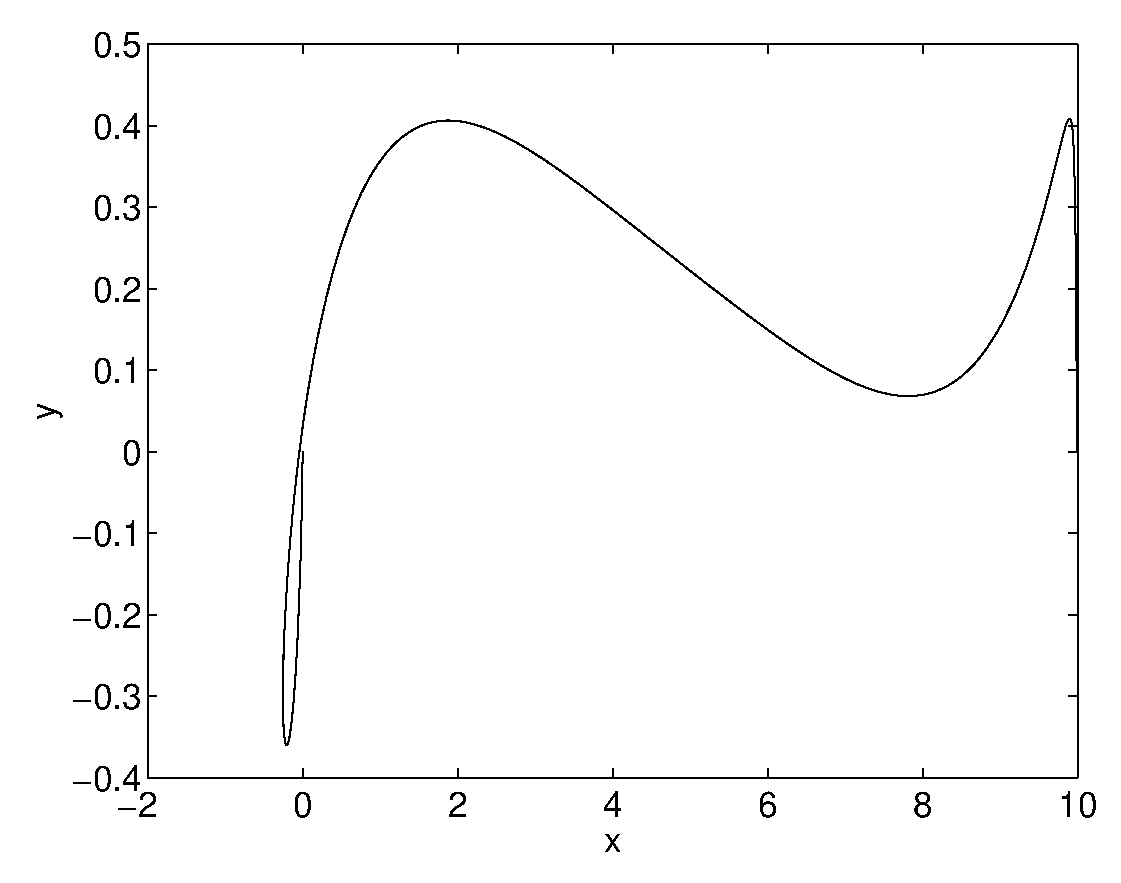
\includegraphics[height=0.3\textheight]{img/final_15_1_10_path.eps}
\caption{path}
\end{subfigure}

\begin{subfigure}[b]{\textwidth}
\centering
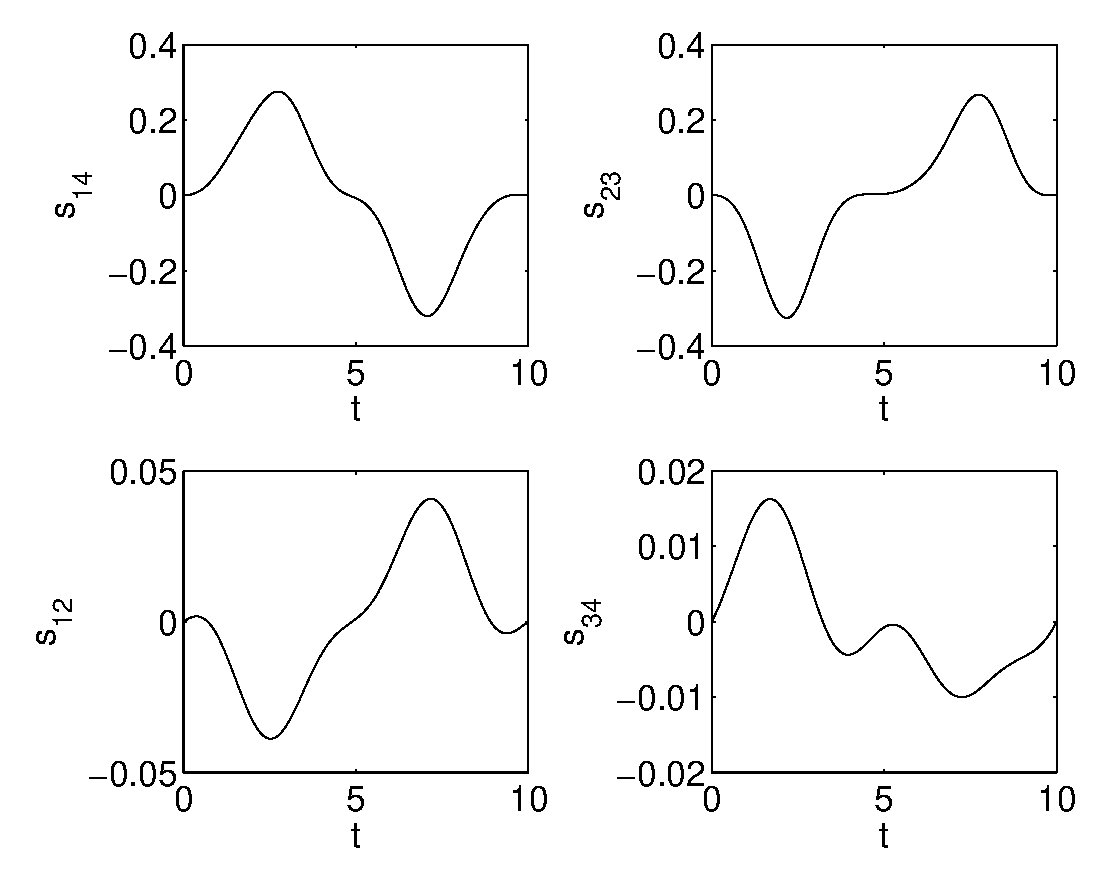
\includegraphics[height=0.3\textheight]{img/final_15_1_10_slips.eps}
\caption{slips}
\end{subfigure}

\begin{subfigure}[b]{\textwidth}
\centering
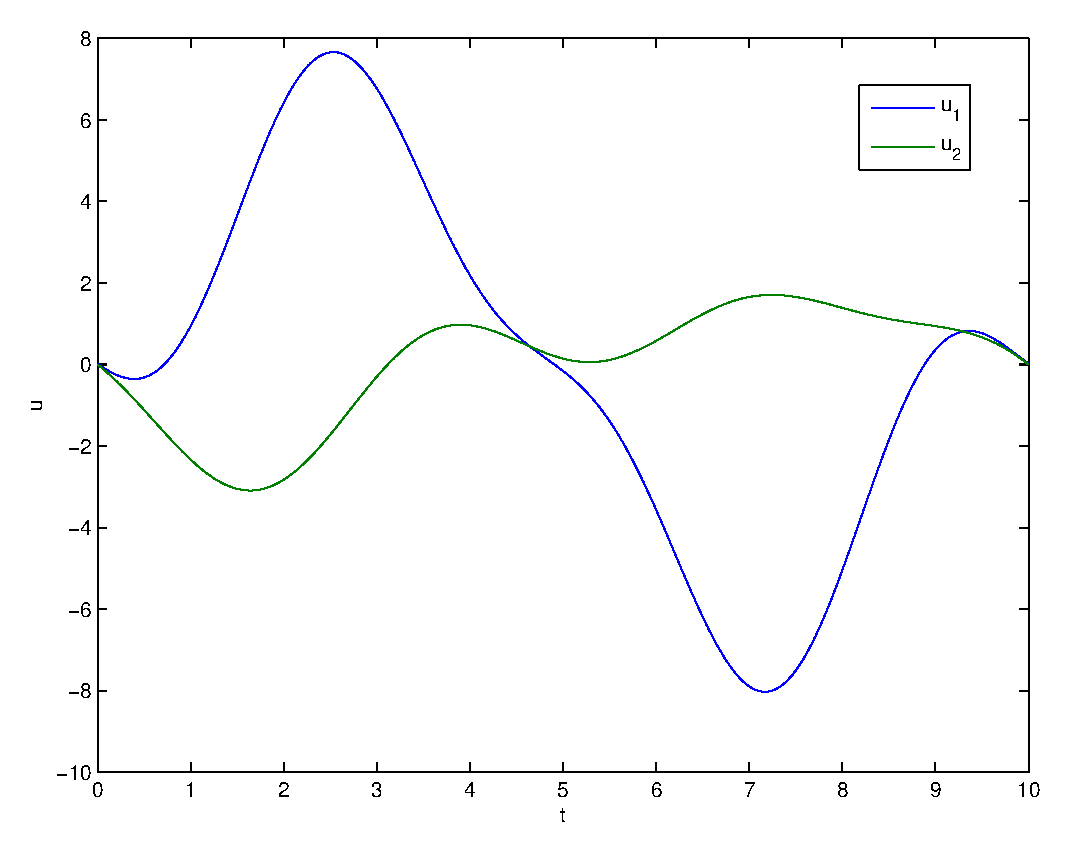
\includegraphics[height=0.3\textheight]{img/final_15_1_10_u.eps}
\caption{path}
\end{subfigure}
\caption{Mobile platform, $\epsilon=15$, $\tau=1$, $T=10$}
\label{fig:pl1}
\end{figure}

\begin{figure}[h]
\begin{subfigure}[b]{\textwidth}
\centering
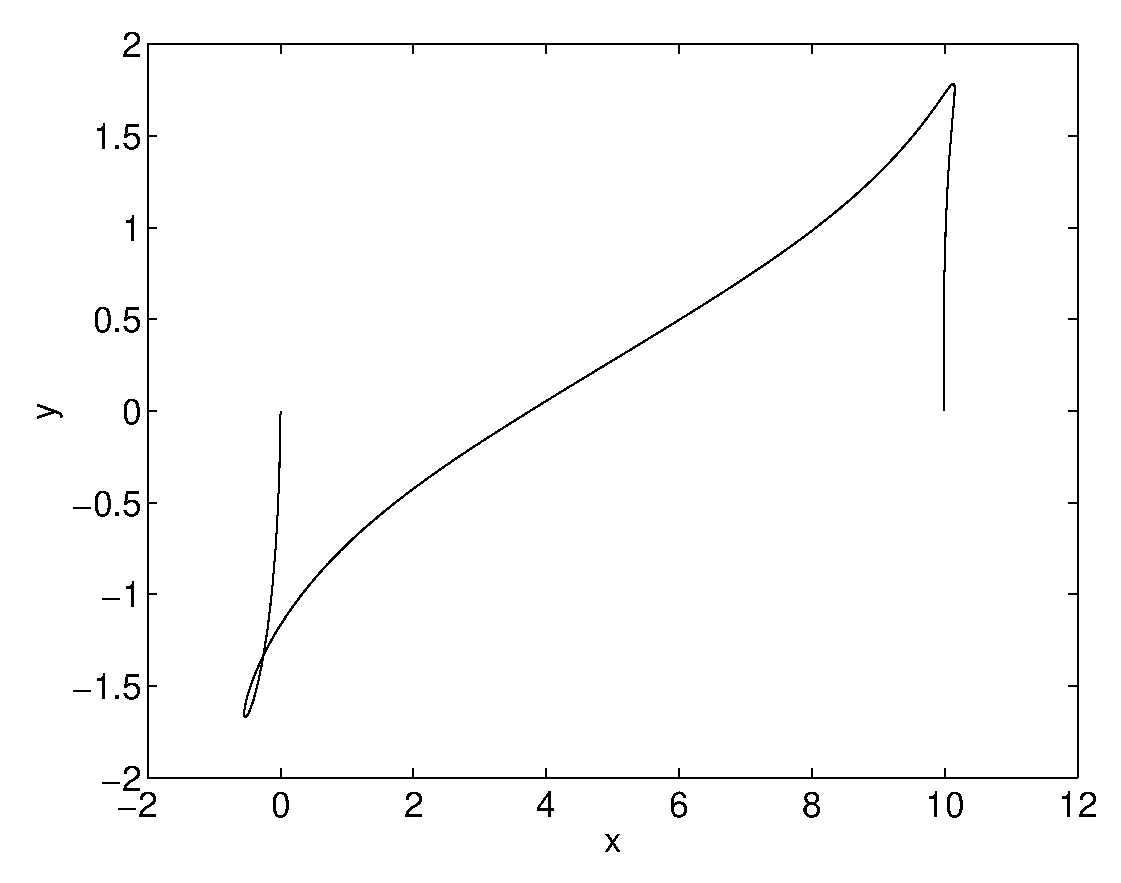
\includegraphics[height=0.3\textheight]{img/final_15_1_20_path.eps}
\caption{path}
\end{subfigure}

\begin{subfigure}[b]{\textwidth}
\centering
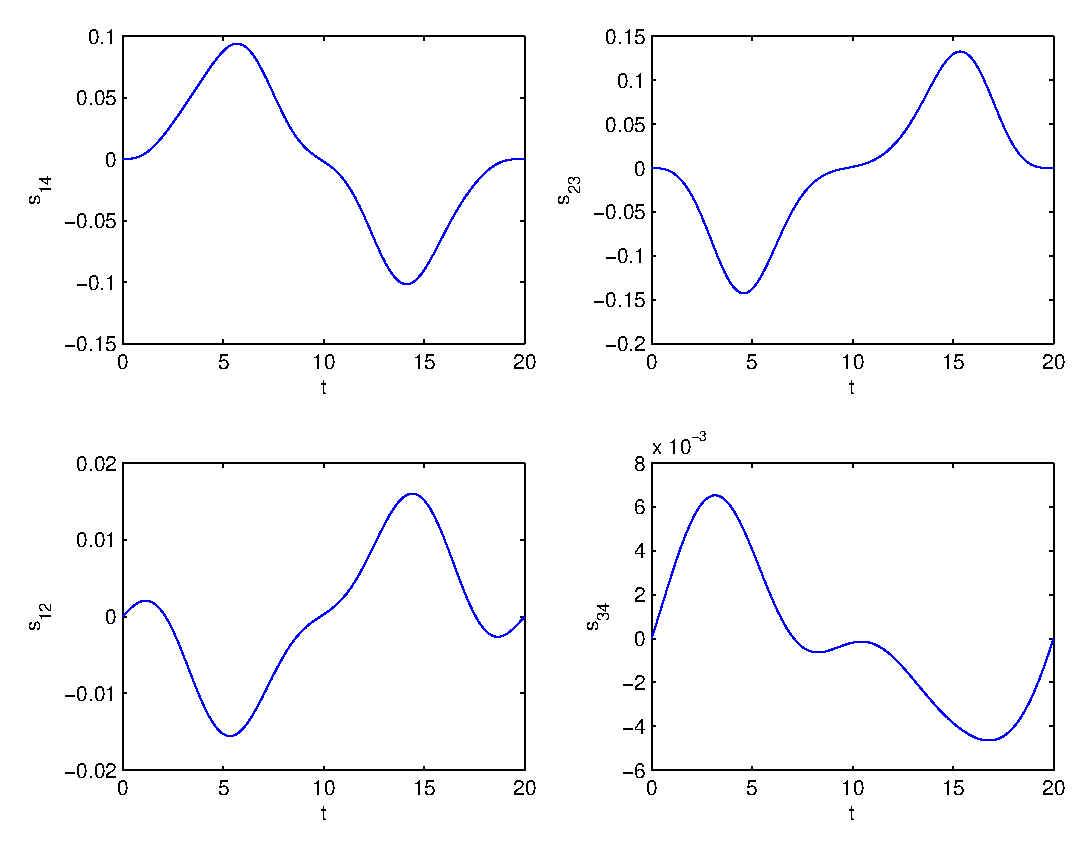
\includegraphics[height=0.3\textheight]{img/final_15_1_20_slips.eps}
\caption{slips}
\end{subfigure}

\begin{subfigure}[b]{\textwidth}
\centering
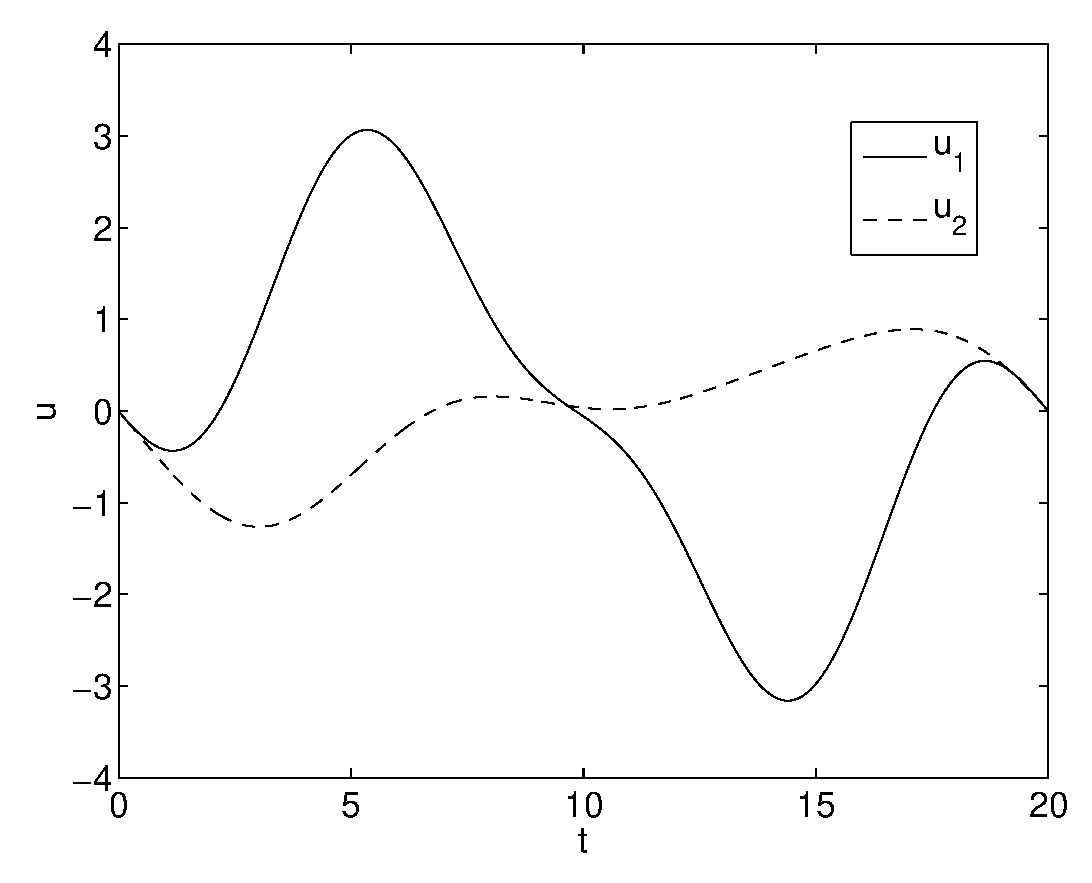
\includegraphics[height=0.3\textheight]{img/final_15_1_20_u.eps}
\caption{path}
\end{subfigure}
\caption{Mobile platform, $\epsilon=15$, $\tau=1$, $T=20$}
\label{fig:pl2}
\end{figure}

%%%%%%%%%%%%%%%%%%%%%%%%%%%%%%%%%%%%%%%%%%%%%%%%%%%%%%%%%%%%%%%%%%%%%%%%%%%%%%%%%%%%%%%%%%%
%%%%%%%%%%%%%%%%%%%%%%%%%%%%%%%%%%%%%%%%%%%%%%%%%%%%%%%%%%%%%%%%%%%%%%%%%%%%%%%%%%%%%%%%%%%
%%%%%%%%%%%%%%%%%%%%%%%%%%%%%%%%%%%%%%%%%%%%%%%%%%%%%%%%%%%%%%%%%%%%%%%%%%%%%%%%%%%%%%%%%%%
%%%%%%%%%%%%%%%%%%%%%%%%%%%%%%%%%%%%%%%%%%%%%%%%%%%%%%%%%%%%%%%%%%%%%%%%%%%%%%%%%%%%%%%%%%%
%%%%%%%%%%%%%%%%%%%%%%%%%%%%%%%%%%%%%%%%%%%%%%%%%%%%%%%%%%%%%%%%%%%%%%%%%%%%%%%%%%%%%%%%%%%

\begin{figure}[h]
\begin{subfigure}[b]{\textwidth}
\centering
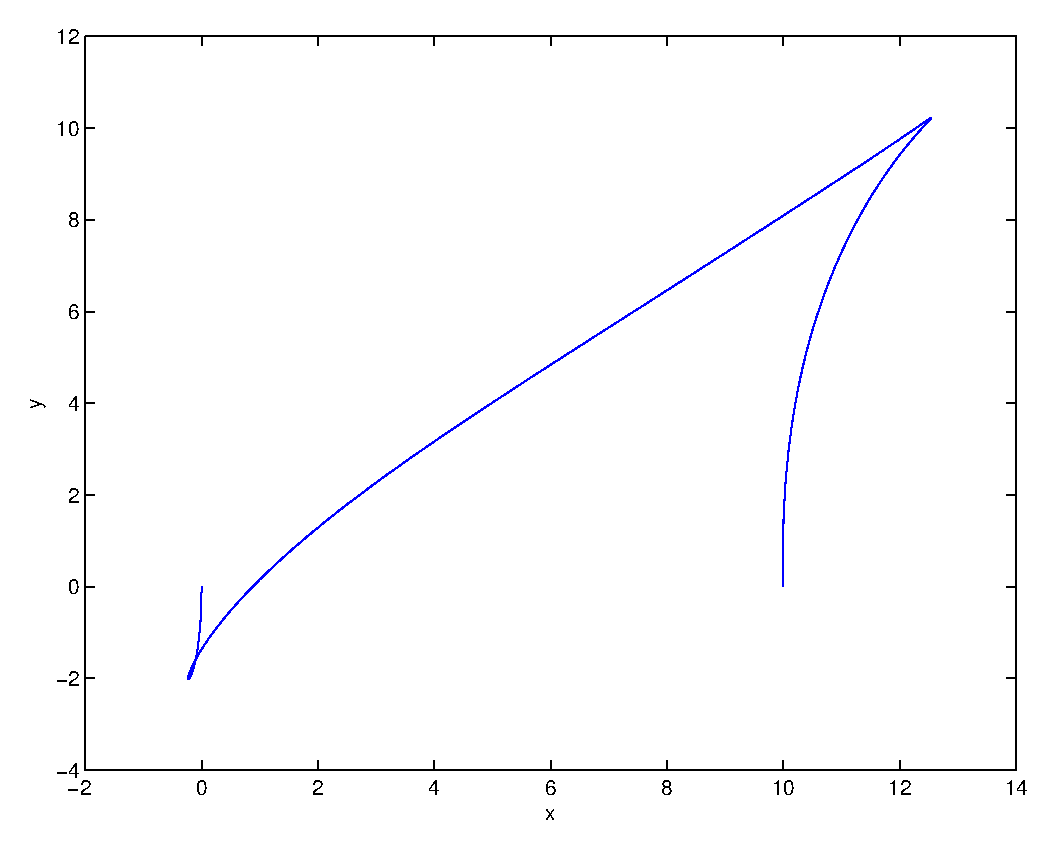
\includegraphics[height=0.3\textheight]{img/final_15_15_10_path.eps}
\caption{path}
\end{subfigure}

\begin{subfigure}[b]{\textwidth}
\centering
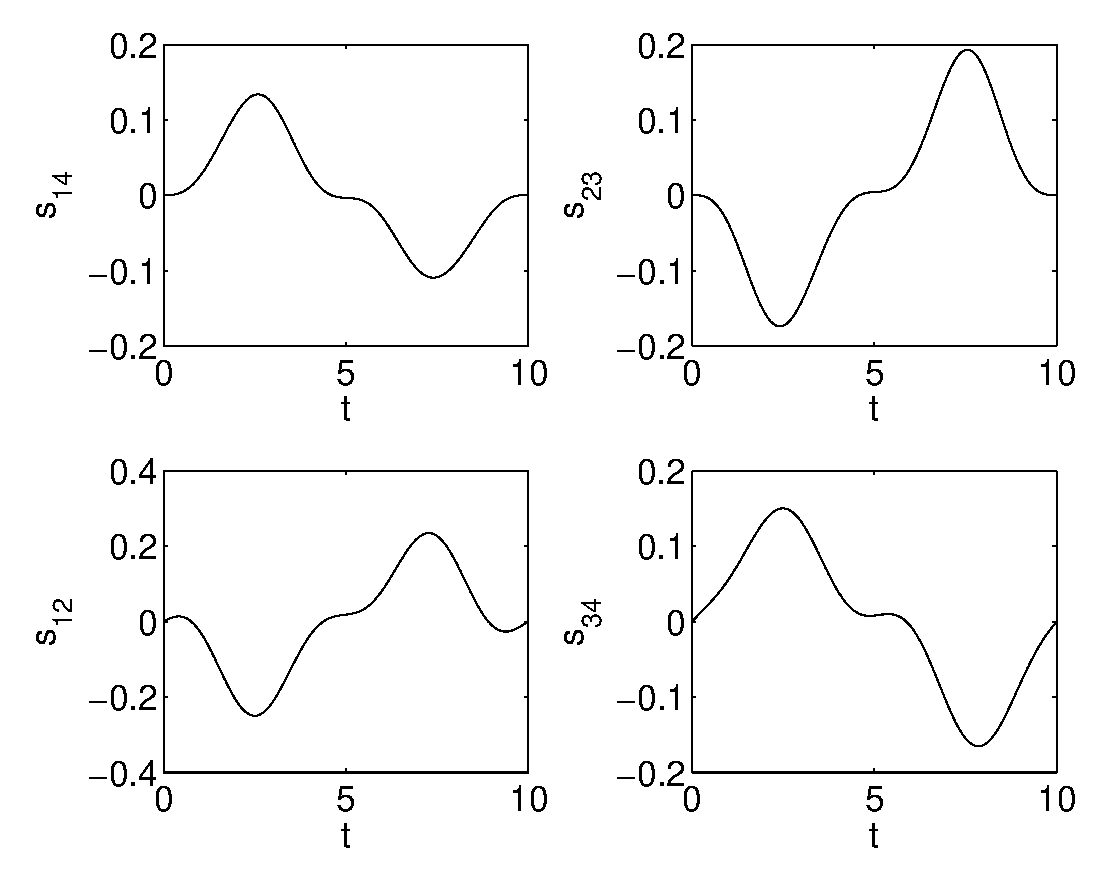
\includegraphics[height=0.3\textheight]{img/final_15_15_10_slips.eps}
\caption{slips}
\end{subfigure}

\begin{subfigure}[b]{\textwidth}
\centering
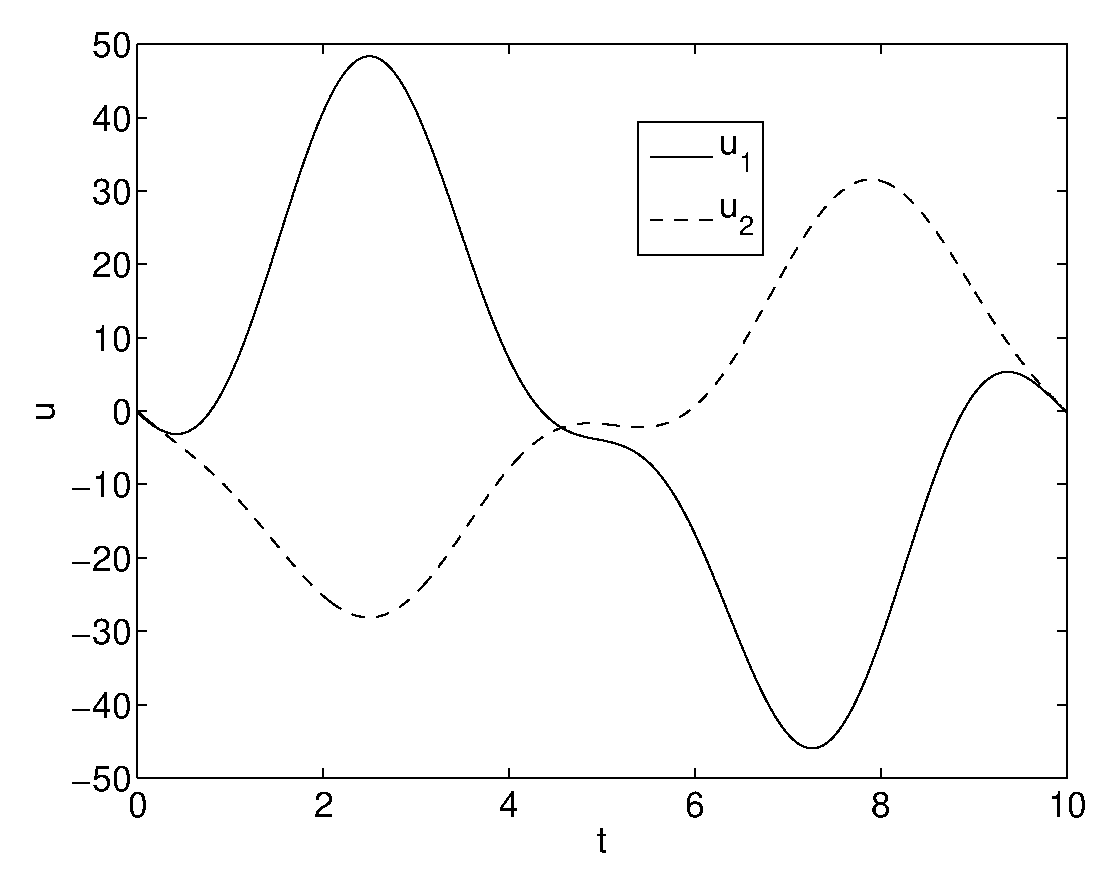
\includegraphics[height=0.3\textheight]{img/final_15_15_10_u.eps}
\caption{path}
\end{subfigure}
\caption{Mobile platform, $\epsilon=15$, $\tau=15$, $T=10$}
\label{fig:pl3}
\end{figure}

\begin{figure}[h]
\begin{subfigure}[b]{\textwidth}
\centering
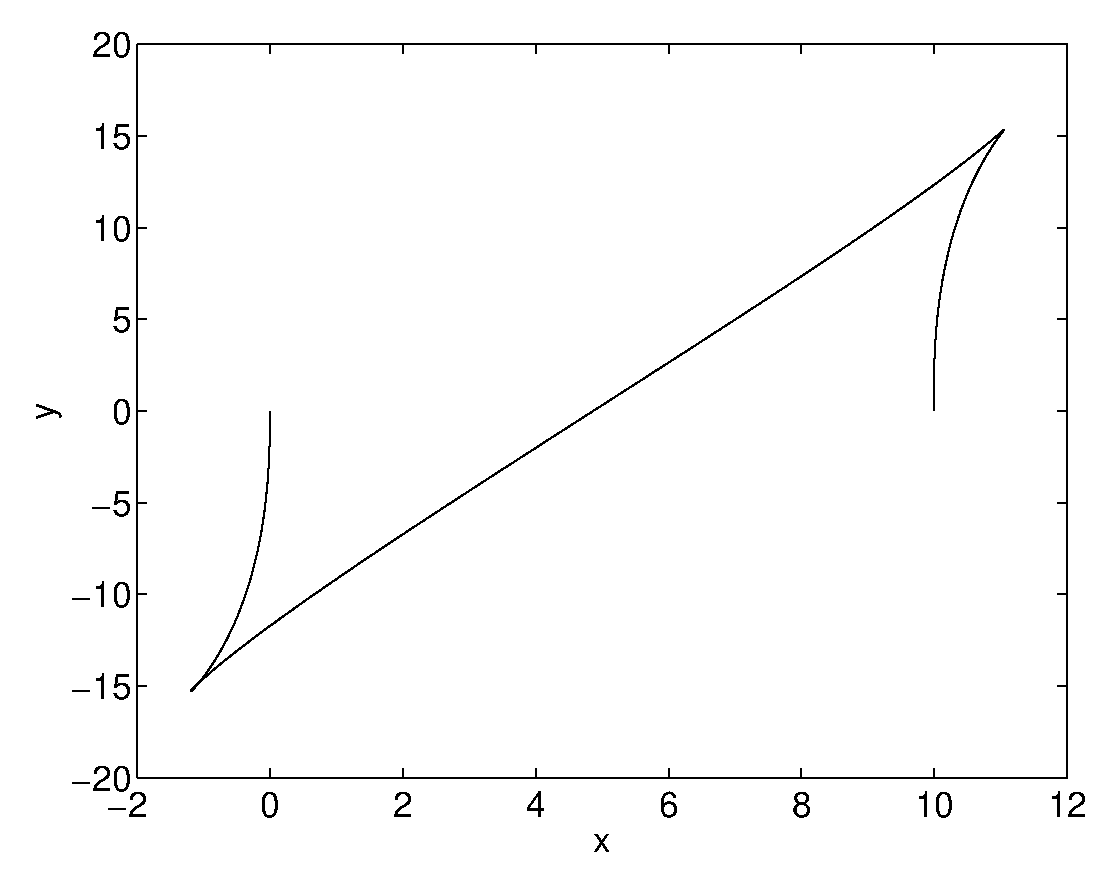
\includegraphics[height=0.3\textheight]{img/final_15_15_20_path.eps}
\caption{path}
\end{subfigure}

\begin{subfigure}[b]{\textwidth}
\centering
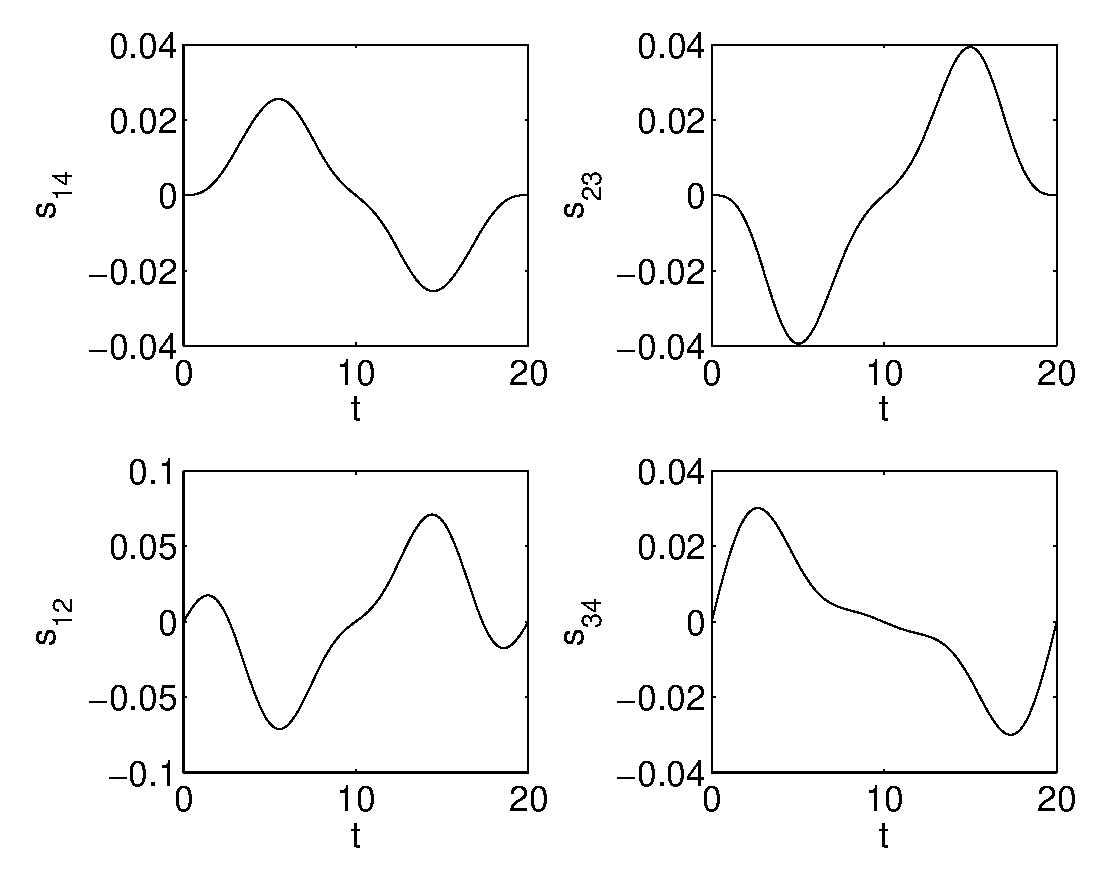
\includegraphics[height=0.3\textheight]{img/final_15_15_20_slips.eps}
\caption{slips}
\end{subfigure}

\begin{subfigure}[b]{\textwidth}
\centering
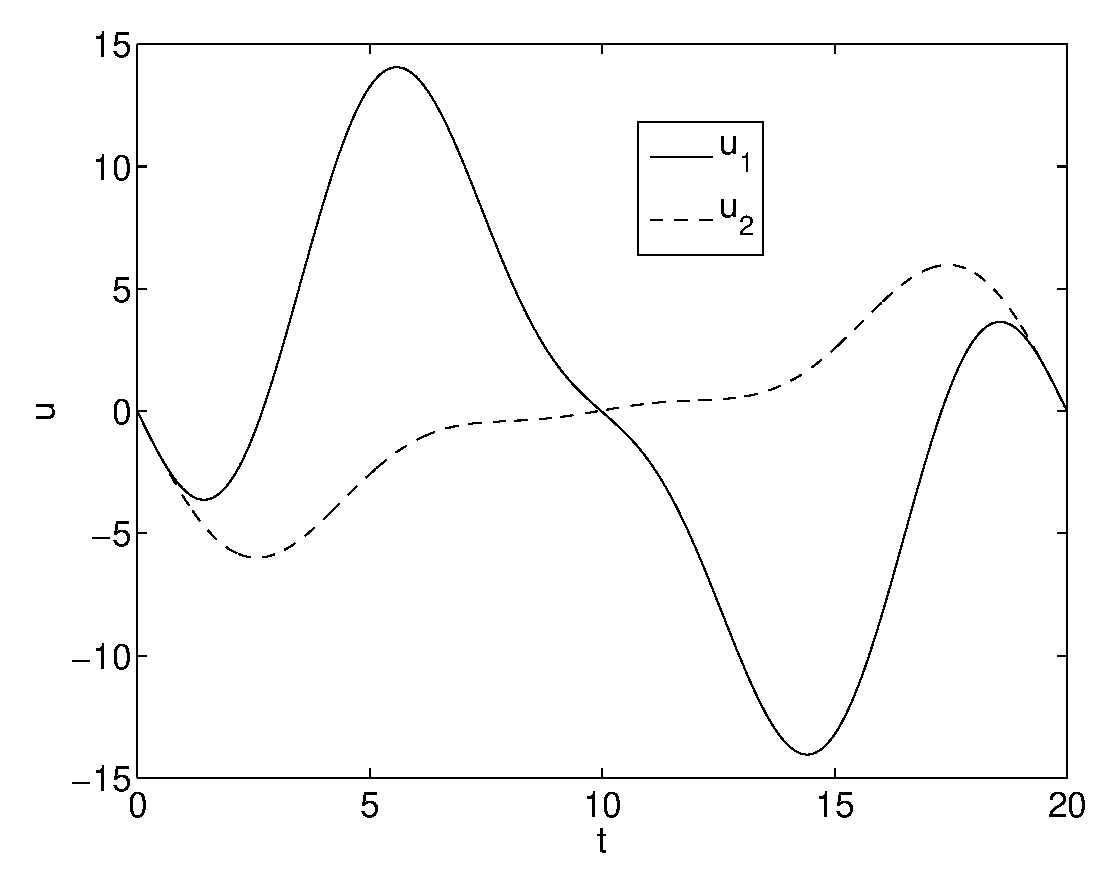
\includegraphics[height=0.3\textheight]{img/final_15_15_20_u.eps}
\caption{path}
\end{subfigure}
\caption{Mobile platform, $\epsilon=15$, $\tau=15$, $T=20$}
\label{fig:pl4}
\end{figure}

%%%%%%%%%%%%%%%%%%%%%%%%%%%%%%%%%%%%%%%%%%%%%%%%%%%%%%%%%%%%%%%%%%%%%%%%%%%%%%%%%%%%%%%%%%%
%%%%%%%%%%%%%%%%%%%%%%%%%%%%%%%%%%%%%%%%%%%%%%%%%%%%%%%%%%%%%%%%%%%%%%%%%%%%%%%%%%%%%%%%%%%
%%%%%%%%%%%%%%%%%%%%%%%%%%%%%%%%%%%%%%%%%%%%%%%%%%%%%%%%%%%%%%%%%%%%%%%%%%%%%%%%%%%%%%%%%%%
%%%%%%%%%%%%%%%%%%%%%%%%%%%%%%%%%%%%%%%%%%%%%%%%%%%%%%%%%%%%%%%%%%%%%%%%%%%%%%%%%%%%%%%%%%%
%%%%%%%%%%%%%%%%%%%%%%%%%%%%%%%%%%%%%%%%%%%%%%%%%%%%%%%%%%%%%%%%%%%%%%%%%%%%%%%%%%%%%%%%%%%
\begin{figure}[h]
\begin{subfigure}[b]{\textwidth}
\centering
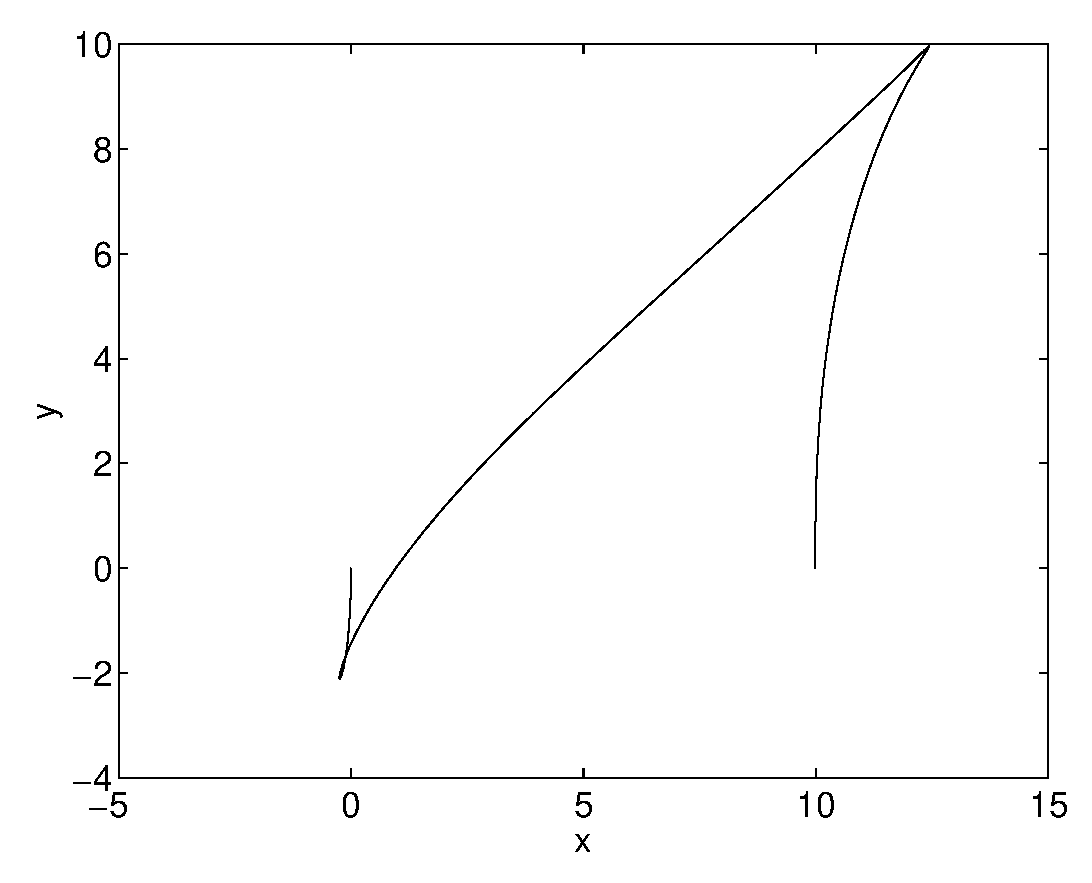
\includegraphics[height=0.3\textheight]{img/final_1_15_10_path.eps}
\caption{path}
\end{subfigure}

\begin{subfigure}[b]{\textwidth}
\centering
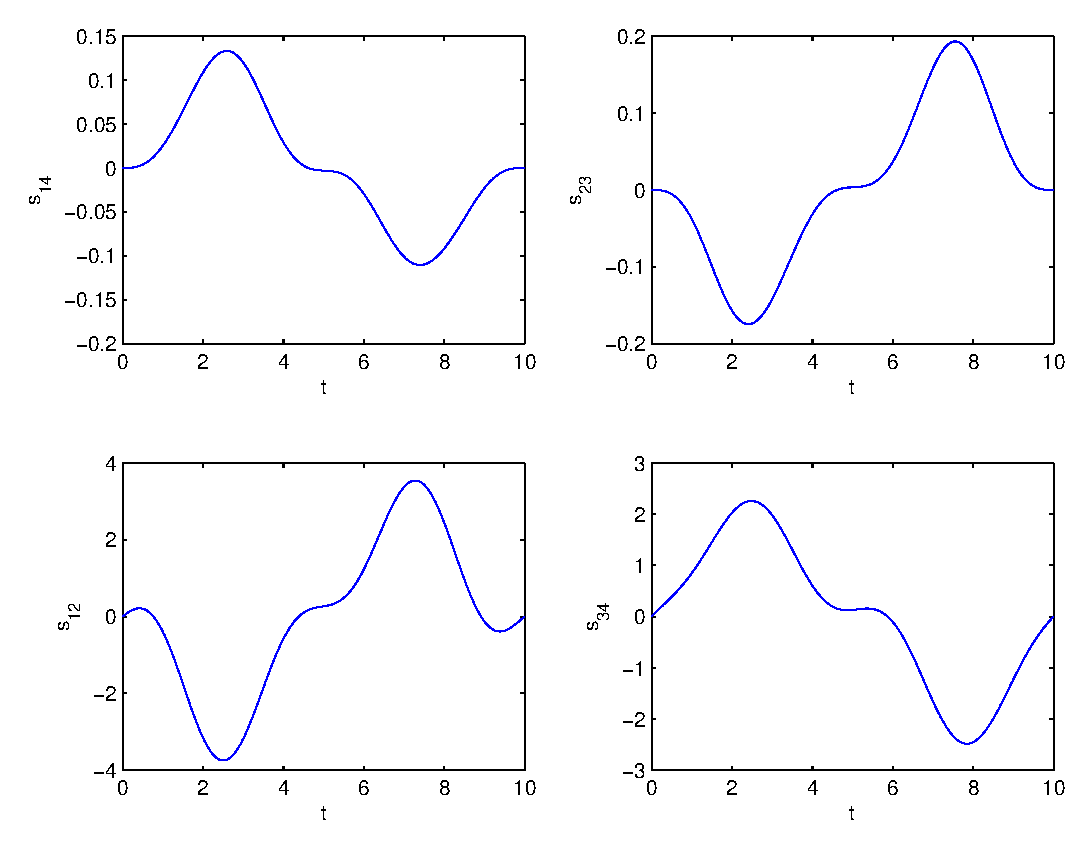
\includegraphics[height=0.3\textheight]{img/final_1_15_10_slips.eps}
\caption{slips}
\end{subfigure}

\begin{subfigure}[b]{\textwidth}
\centering
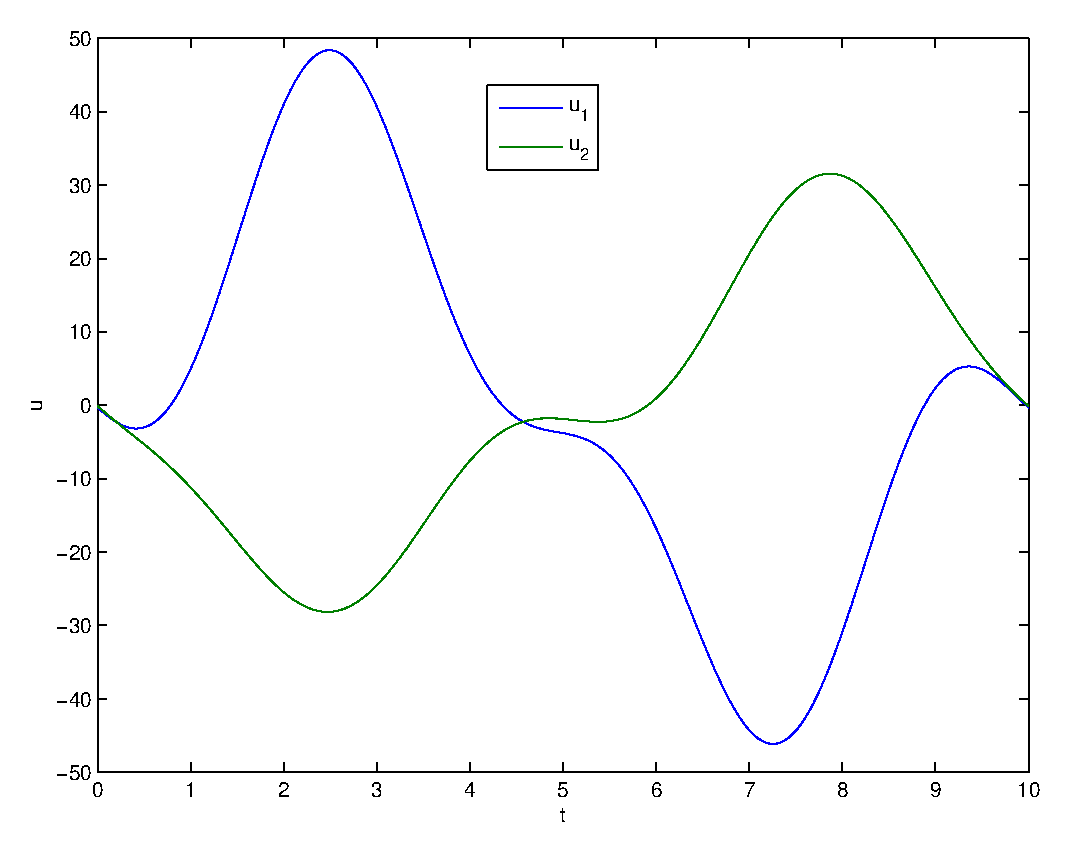
\includegraphics[height=0.3\textheight]{img/final_1_15_10_u.eps}
\caption{path}
\end{subfigure}
\caption{Mobile platform, $\epsilon=1$, $\tau=15$, $T=10$}
\label{fig:pl5}
\end{figure}

\begin{figure}[h]
\begin{subfigure}[b]{\textwidth}
\centering
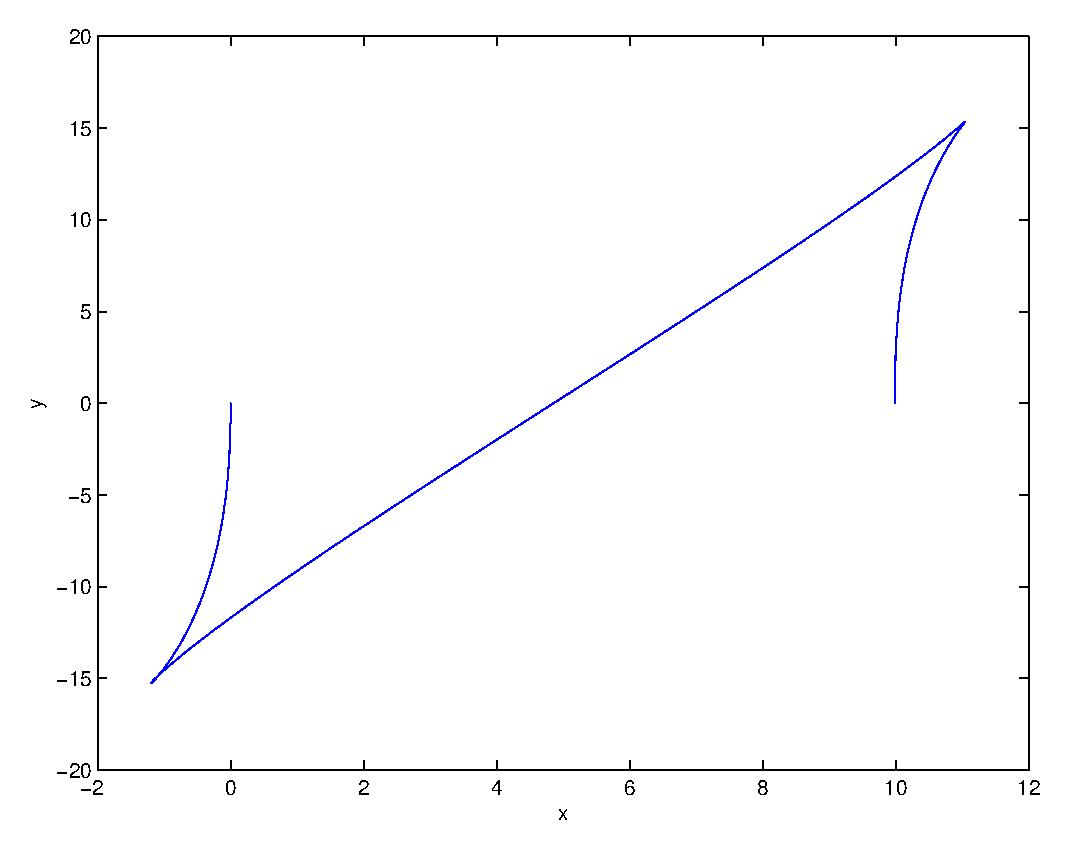
\includegraphics[height=0.3\textheight]{img/final_1_15_20_path.eps}
\caption{path}
\end{subfigure}

\begin{subfigure}[b]{\textwidth}
\centering
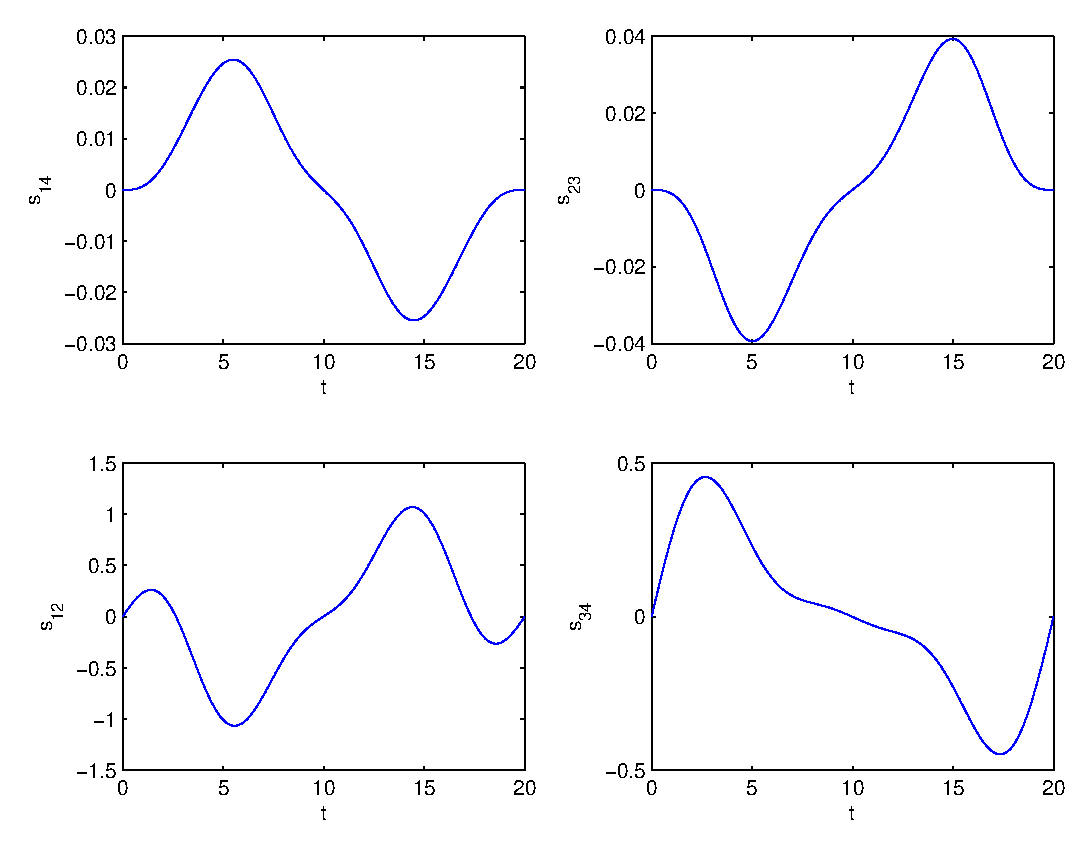
\includegraphics[height=0.3\textheight]{img/final_1_15_20_slips.eps}
\caption{slips}
\end{subfigure}

\begin{subfigure}[b]{\textwidth}
\centering
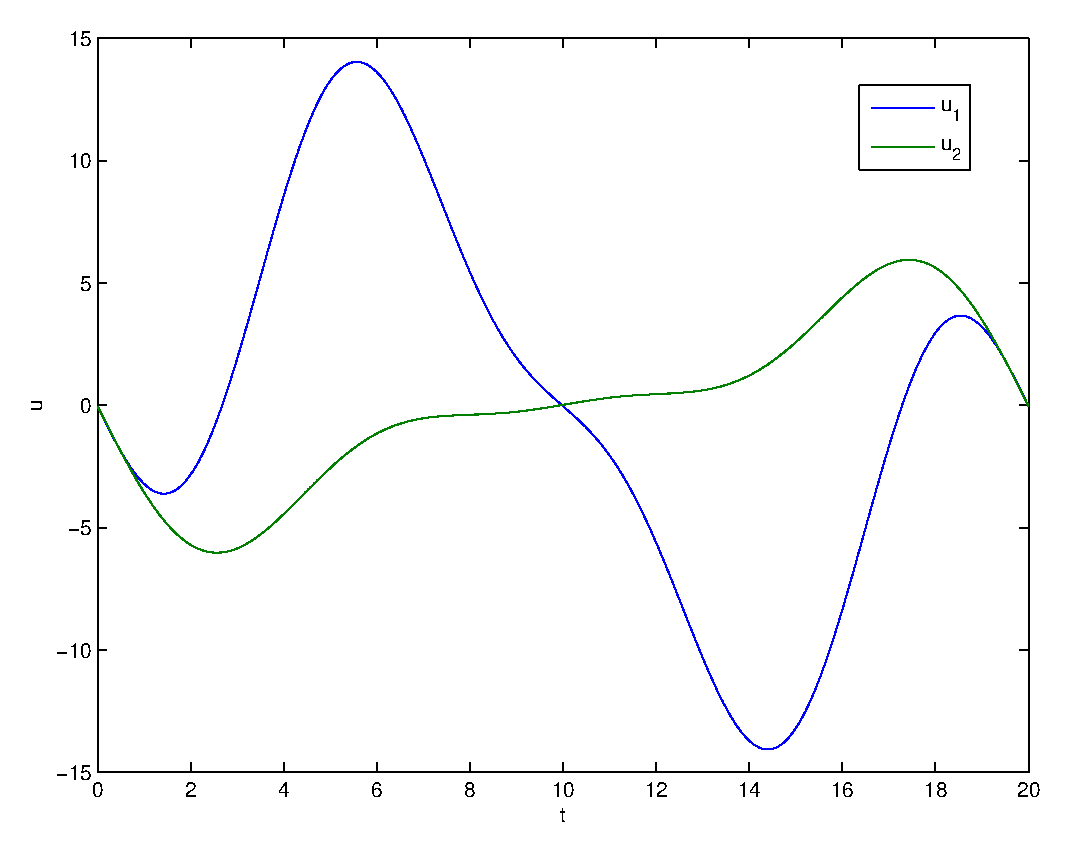
\includegraphics[height=0.3\textheight]{img/final_1_15_20_u.eps}
\caption{path}
\end{subfigure}
\caption{Mobile platform, $\epsilon=1$, $\tau=15$, $T=20$}
\label{fig:pl6}
\end{figure}

%%%%%%%%%%%%%%%%%%%%%%%%%%%%%%%%%%%%%%%%%%%%%%%%%%%%%%%%%%%%%%%%%%%%%%%%%%%%%%%%%%%%%%%%%%%
%%%%%%%%%%%%%%%%%%%%%%%%%%%%%%%%%%%%%%%%%%%%%%%%%%%%%%%%%%%%%%%%%%%%%%%%%%%%%%%%%%%%%%%%%%%
%%%%%%%%%%%%%%%%%%%%%%%%%%%%%%%%%%%%%%%%%%%%%%%%%%%%%%%%%%%%%%%%%%%%%%%%%%%%%%%%%%%%%%%%%%%
%%%%%%%%%%%%%%%%%%%%%%%%%%%%%%%%%%%%%%%%%%%%%%%%%%%%%%%%%%%%%%%%%%%%%%%%%%%%%%%%%%%%%%%%%%%
%%%%%%%%%%%%%%%%%%%%%%%%%%%%%%%%%%%%%%%%%%%%%%%%%%%%%%%%%%%%%%%%%%%%%%%%%%%%%%%%%%%%%%%%%%%
\begin{figure}[h]
\begin{subfigure}[b]{\textwidth}
\centering
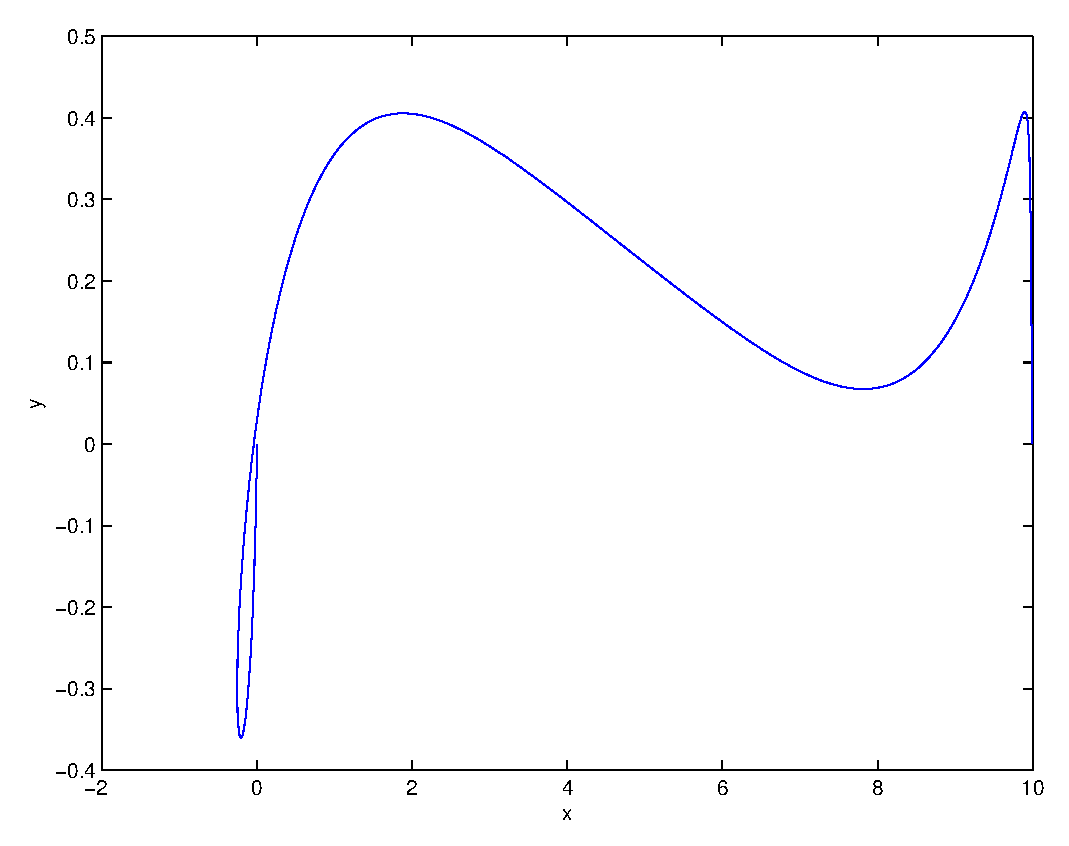
\includegraphics[height=0.3\textheight]{img/final_1_1_10_path.eps}
\caption{path}
\end{subfigure}

\begin{subfigure}[b]{\textwidth}
\centering
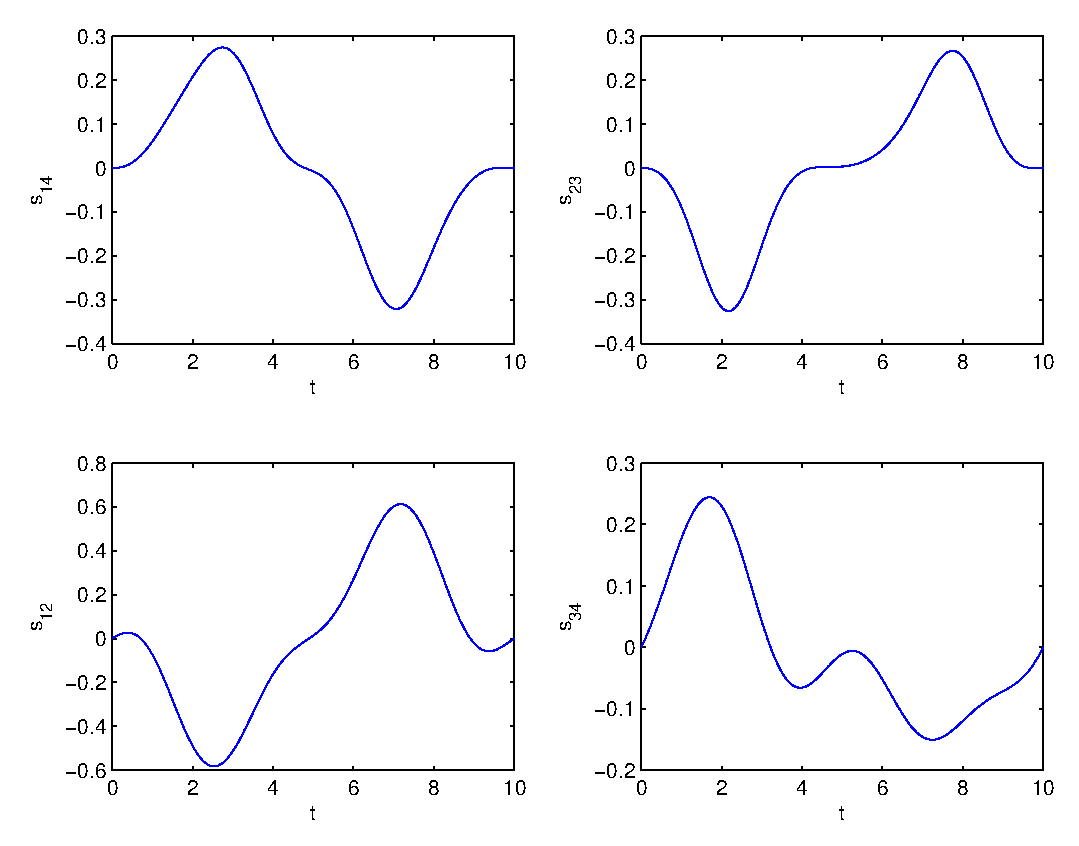
\includegraphics[height=0.3\textheight]{img/final_1_1_10_slips.eps}
\caption{slips}
\end{subfigure}

\begin{subfigure}[b]{\textwidth}
\centering
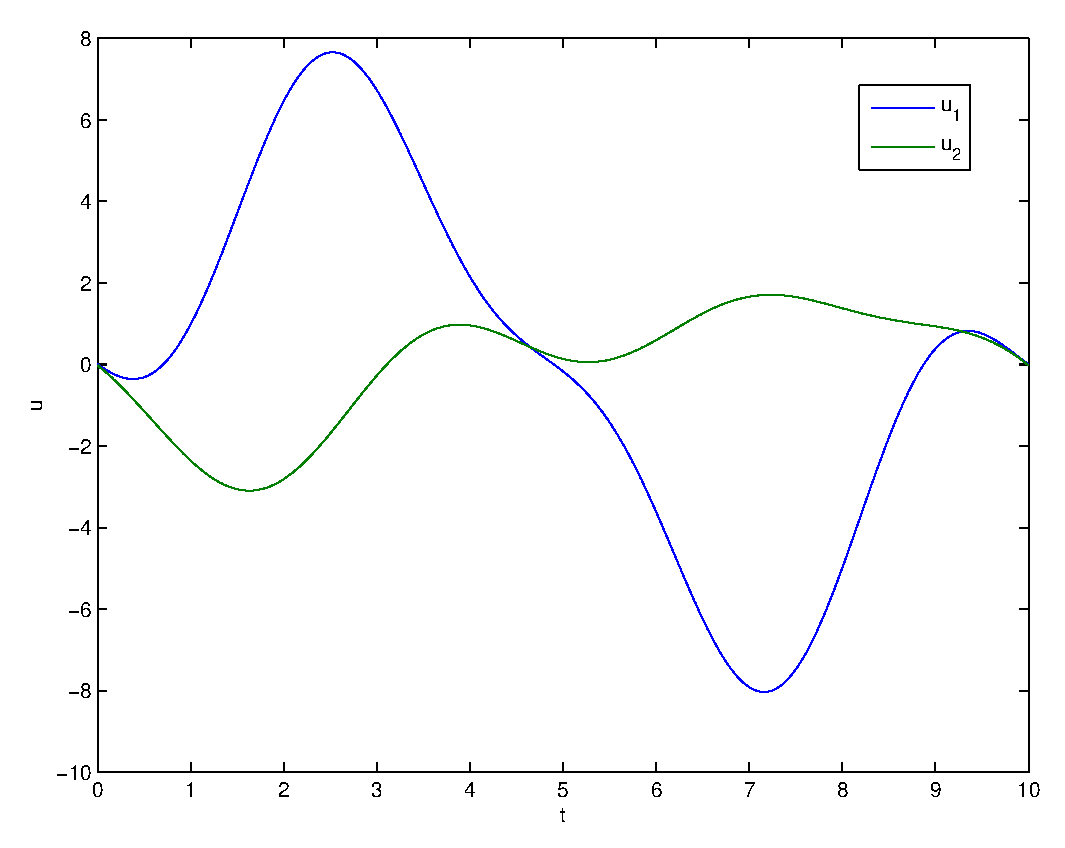
\includegraphics[height=0.3\textheight]{img/final_1_1_10_u.eps}
\caption{path}
\end{subfigure}
\caption{Mobile platform, $\epsilon=1$, $\tau=1$, $T=10$}
\label{fig:pl7}
\end{figure}

\begin{figure}[h]
\begin{subfigure}[b]{\textwidth}
\centering
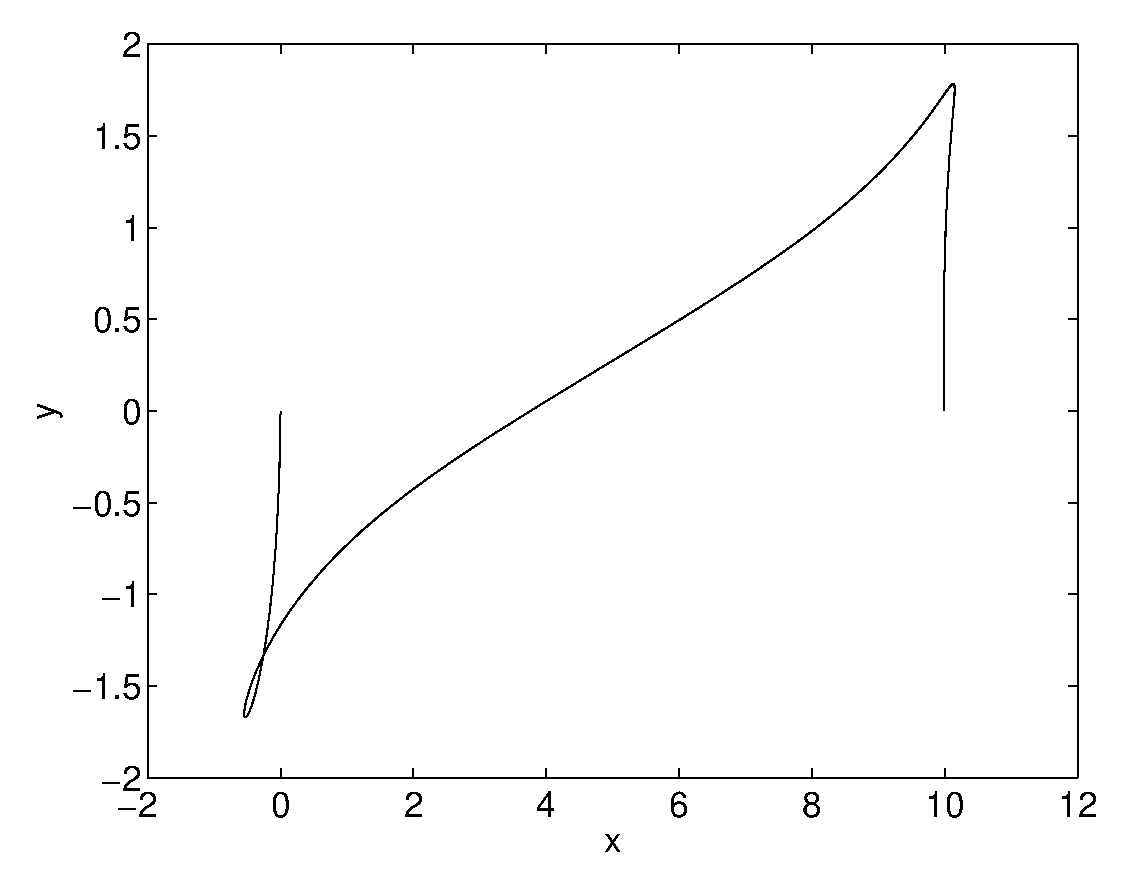
\includegraphics[height=0.3\textheight]{img/final_1_1_20_path.eps}
\caption{path}
\end{subfigure}

\begin{subfigure}[b]{\textwidth}
\centering
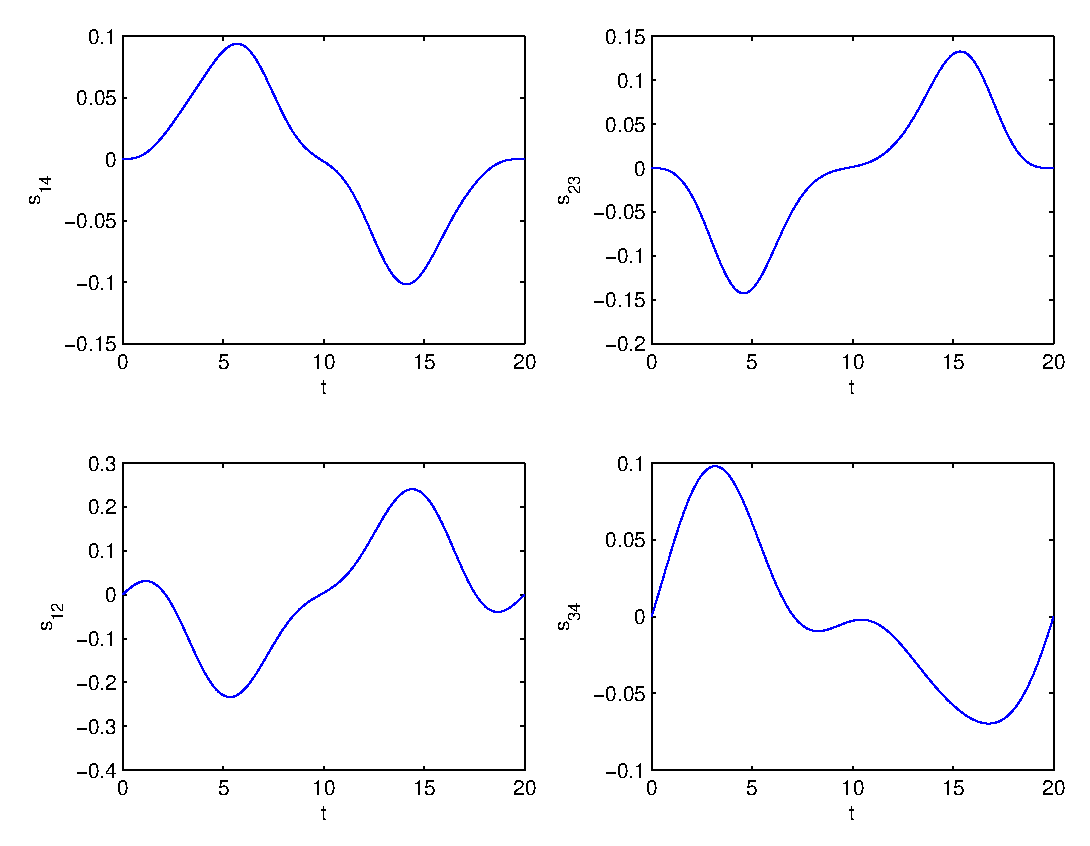
\includegraphics[height=0.3\textheight]{img/final_1_1_20_slips.eps}
\caption{slips}
\end{subfigure}

\begin{subfigure}[b]{\textwidth}
\centering
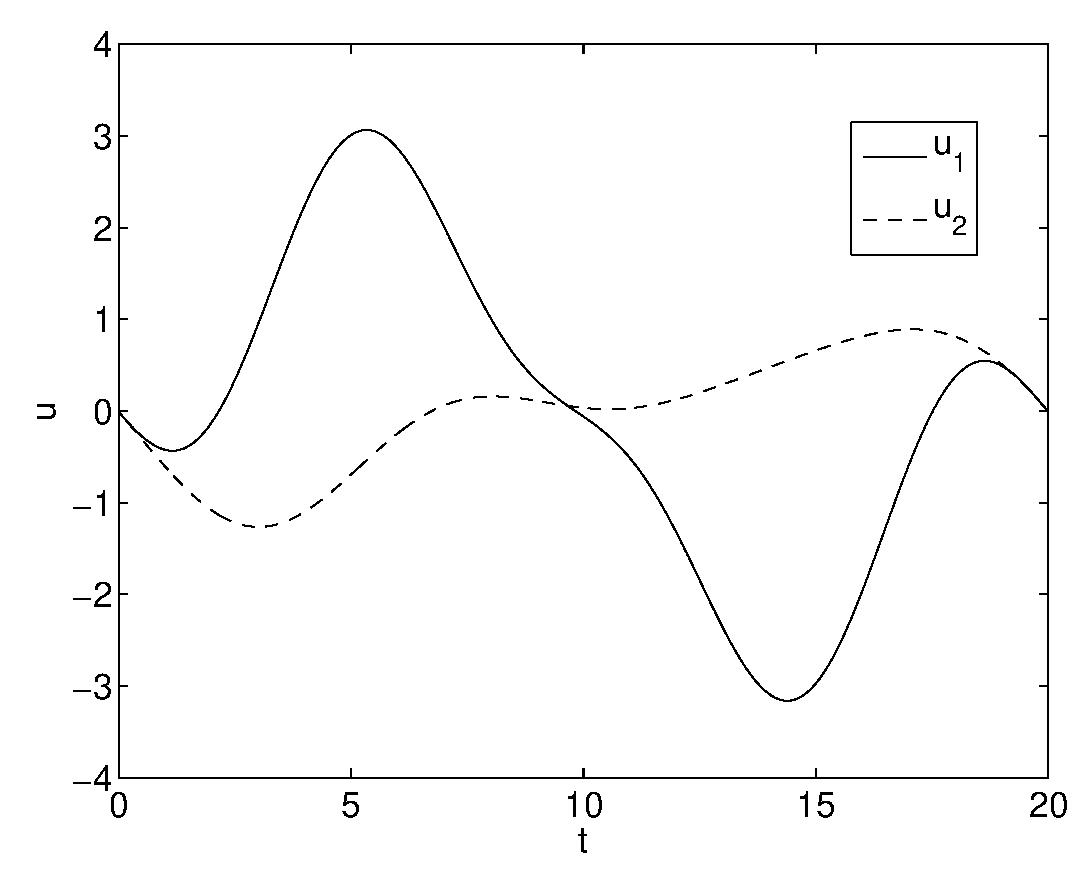
\includegraphics[height=0.3\textheight]{img/final_1_1_20_u.eps}
\caption{path}
\end{subfigure}
\caption{Mobile platform, $\epsilon=1$, $\tau=1$, $T=20$}
\label{fig:pl8}
\end{figure}

%%%%%%%%%%%%%%%%%%%%%%%%%%%%%%%%%%%%%%%%%%%%%%%%%%%%%%%%%%%%%%%%%%%%%%%%%%%%%%%%%%%%%%%%%%%
%%%%%%%%%%%%%%%%%%%%%%%%%%%%%%%%%%%%%%%%%%%%%%%%%%%%%%%%%%%%%%%%%%%%%%%%%%%%%%%%%%%%%%%%%%%
%%%%%%%%%%%%%%%%%%%%%%%%%%%%%%%%%%%%%%%%%%%%%%%%%%%%%%%%%%%%%%%%%%%%%%%%%%%%%%%%%%%%%%%%%%%
%%%%%%%%%%%%%%%%%%%%%%%%%%%%%%%%%%%%%%%%%%%%%%%%%%%%%%%%%%%%%%%%%%%%%%%%%%%%%%%%%%%%%%%%%%%
%%%%%%%%%%%%%%%%%%%%%%%%%%%%%%%%%%%%%%%%%%%%%%%%%%%%%%%%%%%%%%%%%%%%%%%%%%%%%%%%%%%%%%%%%%%

\subsection{Discontinuous friction model}
This model assumes that coefficients $\epsilon_i$ and $\tau_i$ in \eqref{eq:force_r} depend
on the value of the slip. The idea of such friction model has been described
in section \ref{sec:discont_params_uni}. With such an approach the formulae defining
friction coefficients are of the form
\begin{equation*}
\begin{aligned}
\epsilon_1=\epsilon_4&=\begin{cases}
\epsilon_{high} &\mbox{if } |s_{14}| \leq d \\
\epsilon_{low} &\mbox{if } |s_{14}| > d
\end{cases}, &
\tau_1=\tau_2&=\begin{cases}
\tau_{high} &\mbox{if } |s_{12}| \leq d \\
\tau_{low} &\mbox{if } |s_{12}| > d
\end{cases},\\
\epsilon_2=\epsilon_3&=\begin{cases}
\epsilon_{high} &\mbox{if } |s_{23}| \leq d \\
\epsilon_{low} &\mbox{if } |s_{23}| > d
\end{cases}, &
\tau_3=\tau_4&=\begin{cases}
\tau_{high} &\mbox{if } |s_{34}| \leq d \\
\tau_{low} &\mbox{if } |s_{34}| > d
\end{cases}.
\end{aligned}
\end{equation*}
The values used in simulations are: $\epsilon_{high}=10$, $\epsilon_{low}=5$, $\tau_{high}=3$, $\tau_{low}=1$. Unfortunately, there is no guarantee for the algorithm to converge for a discontinuous model and such situation takes place in this case. The plot of the error norm with respect to the iteration number is shown in the figure \ref{fig:error_discont}. It is clearly visible that the plot of the error norm is not monotonic. The reason why the endogenous configuration approach does not perform well here is the fundamental idea of the motion planning algorithm. It assumes that a small change in endogenous configuration results in a small change in the output function value. This statement is true for continuous models. On the contrary, when a model includes some discontinuities, even a small variation to the input may take the system to a distant point from the original one in the output space. Therefore, the error may increase in the next iteration of the algorithm. Note that decreasing the $\gamma$ parameter in equation \eqref{eq:endogen_num} will not solve this problem neither.
In other words, if the platform loses the traction in a different point than in
the previous iteration it ends up in a place not related to the one supposed to be
according to the algorithm, because actually the model has changed in the meanwhile.
\begin{figure}[htp]
\centering
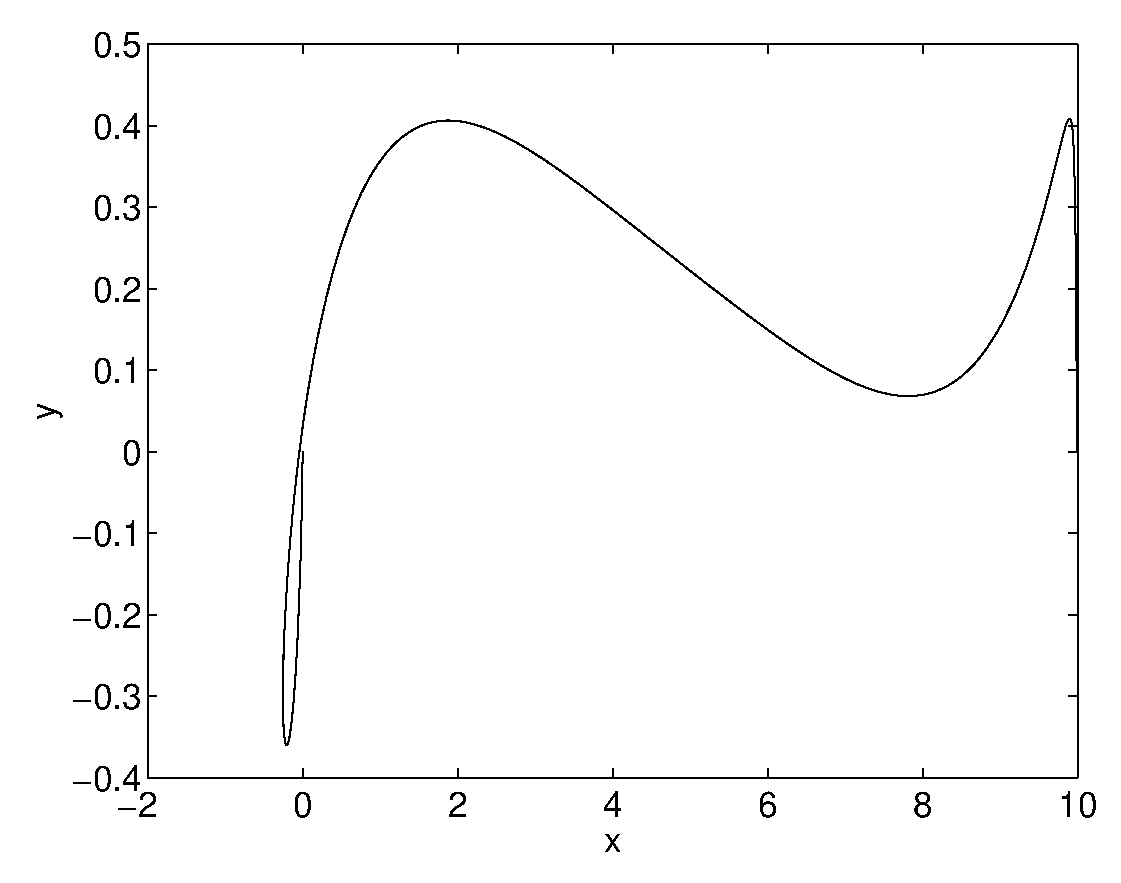
\includegraphics[height=0.3\textheight]{img/final_15_1_10_path.eps} %TODO make proper image
\caption{Error norm w.r.t iteration, discontinuous model of the platform}
\label{fig:error_discont}
\end{figure}

\section{Mobile manipulator}
This section covers the simulations for the whole RobRex mobile manipulator. Two types of problems will
be discussed here: with constraints only for the end-effector configuration and with constraints for
both mobile platform and the effector.
\subsection{Problems formulation}
The initial conditions for both tasks are: $q_0 = [w_0; \dot{w}_0] = (0, 0, a\frac{\pi}{2}, 0_7)^T$, 
$x_0 = \left(
x_1 ,\, x_2 ,\, x_4 ,\, x_5
\right) = \left(
\frac{\pi}{4} ,\, \frac{\pi}{5} ,\, \frac{\pi}{6} ,\, -\frac{\pi}{3}
\right).$ The control horizon for these tasks is $T=20\,\mathrm{s}$.
\subsubsection{Problem one}
This motion planning problem regards only the end position of the effector
and the velocities of the platform. 
The coordinates in global task space $(x, y, z, \phi, \theta, \psi) $ should be equal to
$(10, 0, 0.2, \frac{\pi}{2}, \frac{\pi}{4}, -\frac{\pi}{2})$. The velocity of each platform coordinate
should be equal to zero. Such constraints guarantee that the whole system will stand still at the end
of the motion.
\subsubsection{Problem two}
This case is related to the platform pose as well as to the configuration of the effector.
As far as the platform is concerned, the constraints are put only on the $x$ coordinate and
the velocities. The desired values are $(x_p, \dot{w}) = (10, 0, 0, 0, 0, 0)$. When it comes to
the effector, the we want the following set of coordinate in global task space: $(y, \phi, \theta, \psi)
= (0, \frac{\pi}{2}, \frac{\pi}{4}, -\frac{\pi}{2})$.

\subsection{Simulation conditions}
The platform parameter has been set as in section \ref{sec:pltf_params}. The lenghts of the links
are equal to:
\begin{multicols}{2}
\begin{itemize}
\item $a_2=0.1276 \,\mathrm{m}$,
\item $a_3=0.041 \,\mathrm{m}$,
\item $a_4=0.2615 \,\mathrm{m}$,
\item $a_5=0.0195 \,\mathrm{m}$.
\end{itemize}
\end{multicols}
First and second joint of the manipulator are actually in the same place, so we assume that $a_1=0$.

\subsection{Simulation results}
The outcome of the simulations are presented in figure \ref{fig:pr1} for the problem one and in figure
\ref{fig:pr2} for the problem two. These figures include the plots of the error with respect to the
iteration, the platform path, the slips values and the inputs. The angles computed for joints are
presented in table \ref{tab:effector}. Regarding the control inputs parameters, table \ref{tab:in_eff}
shows the total energy values of the signal and the maximum amplitudes.

\chapter{Conclusions}
\label{ch:concl}
This work was intended to illustrate the performance of the motion planning algorithm
basing on the endogenous configuration space approach. This method is based on Jacobian,
similarly to the inverse kinematics algorithms, so there may occur problems with
singularity.
The research has been made 
using two models --- a unicycle and RobRex mobile manipulator. First of them was investigated
on a dynamical level and the latter was studied as a separate mobile platform and as the whole.

The algorithm used in this paper behaved well for the continuous model of the mobile platform
as well as for the mobile manipulator and always produced a valid result.
It has been noticed that the friction coefficients which
define the slips configuration play an important role for the outcome of the computations.
For a mobile robot with all fixed-axis wheels it is necessary to skid in the lateral direction
in order to turn. For this reason, the parameters of the results obtained with low lateral friction
coefficients were better. This has a few consequences. First of all, the total area needed to
complete the manoeuvre was far less in these cases. Setting high lateral friction
coefficients makes the robot harder to turn and may even lead to singular configurations.
This phenomenon is reflected also by the value of the dexterity matrix determinant.
Apart from this issue, the lateral friction coefficients have great impact to the values
of the control functions, regarding their energy and amplitude. High friction may cause
the input very high that it can become unobtainable for actuators.

The next aspect making the inputs large is the control horizon. It has been observed that shortening
it two times makes the amplitude of the input about three times greater. Similar effect is obsereved
for the total energy of the control signal.

The advantage of the algorithm is that it may be used for planning the motion with respect
to the effector position. It has been shown that the control of the platform and the configuration
of the manipulator may be determined simultaneously what results in a desired effector configuration.
The output function defining the desired state of the system may also include constraints
for the state of the platform unless it is physically feasible by the controlled object.

However, the important purpose of the research was to examine
this planning method applied to a discontinuous model.
In order to implement the simulations of the discontinuous model it is convenient to use the event
mechanism from MATLAB. It allows to stop the simulation when a discontinuity is detected, save the state
of the object and then start next simulation with a new switched model assuming the initial conditions
the same as the terminal ones from the previous computations.

The conclusion is that endogenous configuration approach does not work
in general, but some special cases may be found that the algorithm figures out useful results.
Broadly speaking, the result is positive when the changes at discontinuities are not
large. Two sets of friction coefficients has been tested and the algorithm
converged only in the case when the difference introduced by switching the model was little.
This is happening because the fundamental idea of the endogenous configurations approach
bases on the fact that small change to the control input induces a small change to the output function.
Assuming that we use Jacobian method to determine the direction of the input, we modify the endogenous
configuration in order to move the object nearer to the desired state. If the model contains
discontinuities, such modification may lead in the wrong direction and the algorithm does not converge.

\bibliography{library}
\bibliographystyle{unsrt}

\end{document}
%  LocalWords:  RTT
